% Options for packages loaded elsewhere
\PassOptionsToPackage{unicode}{hyperref}
\PassOptionsToPackage{hyphens}{url}
%
\documentclass[
]{article}
\usepackage{lmodern}
\usepackage{amssymb,amsmath}
\usepackage{ifxetex,ifluatex}
\ifnum 0\ifxetex 1\fi\ifluatex 1\fi=0 % if pdftex
  \usepackage[T1]{fontenc}
  \usepackage[utf8]{inputenc}
  \usepackage{textcomp} % provide euro and other symbols
\else % if luatex or xetex
  \usepackage{unicode-math}
  \defaultfontfeatures{Scale=MatchLowercase}
  \defaultfontfeatures[\rmfamily]{Ligatures=TeX,Scale=1}
\fi
% Use upquote if available, for straight quotes in verbatim environments
\IfFileExists{upquote.sty}{\usepackage{upquote}}{}
\IfFileExists{microtype.sty}{% use microtype if available
  \usepackage[]{microtype}
  \UseMicrotypeSet[protrusion]{basicmath} % disable protrusion for tt fonts
}{}
\makeatletter
\@ifundefined{KOMAClassName}{% if non-KOMA class
  \IfFileExists{parskip.sty}{%
    \usepackage{parskip}
  }{% else
    \setlength{\parindent}{0pt}
    \setlength{\parskip}{6pt plus 2pt minus 1pt}}
}{% if KOMA class
  \KOMAoptions{parskip=half}}
\makeatother
\usepackage{xcolor}
\IfFileExists{xurl.sty}{\usepackage{xurl}}{} % add URL line breaks if available
\IfFileExists{bookmark.sty}{\usepackage{bookmark}}{\usepackage{hyperref}}
\hypersetup{
  pdftitle={Proposal Analysis},
  hidelinks,
  pdfcreator={LaTeX via pandoc}}
\urlstyle{same} % disable monospaced font for URLs
\usepackage[margin=1in]{geometry}
\usepackage{color}
\usepackage{fancyvrb}
\newcommand{\VerbBar}{|}
\newcommand{\VERB}{\Verb[commandchars=\\\{\}]}
\DefineVerbatimEnvironment{Highlighting}{Verbatim}{commandchars=\\\{\}}
% Add ',fontsize=\small' for more characters per line
\usepackage{framed}
\definecolor{shadecolor}{RGB}{248,248,248}
\newenvironment{Shaded}{\begin{snugshade}}{\end{snugshade}}
\newcommand{\AlertTok}[1]{\textcolor[rgb]{0.94,0.16,0.16}{#1}}
\newcommand{\AnnotationTok}[1]{\textcolor[rgb]{0.56,0.35,0.01}{\textbf{\textit{#1}}}}
\newcommand{\AttributeTok}[1]{\textcolor[rgb]{0.77,0.63,0.00}{#1}}
\newcommand{\BaseNTok}[1]{\textcolor[rgb]{0.00,0.00,0.81}{#1}}
\newcommand{\BuiltInTok}[1]{#1}
\newcommand{\CharTok}[1]{\textcolor[rgb]{0.31,0.60,0.02}{#1}}
\newcommand{\CommentTok}[1]{\textcolor[rgb]{0.56,0.35,0.01}{\textit{#1}}}
\newcommand{\CommentVarTok}[1]{\textcolor[rgb]{0.56,0.35,0.01}{\textbf{\textit{#1}}}}
\newcommand{\ConstantTok}[1]{\textcolor[rgb]{0.00,0.00,0.00}{#1}}
\newcommand{\ControlFlowTok}[1]{\textcolor[rgb]{0.13,0.29,0.53}{\textbf{#1}}}
\newcommand{\DataTypeTok}[1]{\textcolor[rgb]{0.13,0.29,0.53}{#1}}
\newcommand{\DecValTok}[1]{\textcolor[rgb]{0.00,0.00,0.81}{#1}}
\newcommand{\DocumentationTok}[1]{\textcolor[rgb]{0.56,0.35,0.01}{\textbf{\textit{#1}}}}
\newcommand{\ErrorTok}[1]{\textcolor[rgb]{0.64,0.00,0.00}{\textbf{#1}}}
\newcommand{\ExtensionTok}[1]{#1}
\newcommand{\FloatTok}[1]{\textcolor[rgb]{0.00,0.00,0.81}{#1}}
\newcommand{\FunctionTok}[1]{\textcolor[rgb]{0.00,0.00,0.00}{#1}}
\newcommand{\ImportTok}[1]{#1}
\newcommand{\InformationTok}[1]{\textcolor[rgb]{0.56,0.35,0.01}{\textbf{\textit{#1}}}}
\newcommand{\KeywordTok}[1]{\textcolor[rgb]{0.13,0.29,0.53}{\textbf{#1}}}
\newcommand{\NormalTok}[1]{#1}
\newcommand{\OperatorTok}[1]{\textcolor[rgb]{0.81,0.36,0.00}{\textbf{#1}}}
\newcommand{\OtherTok}[1]{\textcolor[rgb]{0.56,0.35,0.01}{#1}}
\newcommand{\PreprocessorTok}[1]{\textcolor[rgb]{0.56,0.35,0.01}{\textit{#1}}}
\newcommand{\RegionMarkerTok}[1]{#1}
\newcommand{\SpecialCharTok}[1]{\textcolor[rgb]{0.00,0.00,0.00}{#1}}
\newcommand{\SpecialStringTok}[1]{\textcolor[rgb]{0.31,0.60,0.02}{#1}}
\newcommand{\StringTok}[1]{\textcolor[rgb]{0.31,0.60,0.02}{#1}}
\newcommand{\VariableTok}[1]{\textcolor[rgb]{0.00,0.00,0.00}{#1}}
\newcommand{\VerbatimStringTok}[1]{\textcolor[rgb]{0.31,0.60,0.02}{#1}}
\newcommand{\WarningTok}[1]{\textcolor[rgb]{0.56,0.35,0.01}{\textbf{\textit{#1}}}}
\usepackage{graphicx,grffile}
\makeatletter
\def\maxwidth{\ifdim\Gin@nat@width>\linewidth\linewidth\else\Gin@nat@width\fi}
\def\maxheight{\ifdim\Gin@nat@height>\textheight\textheight\else\Gin@nat@height\fi}
\makeatother
% Scale images if necessary, so that they will not overflow the page
% margins by default, and it is still possible to overwrite the defaults
% using explicit options in \includegraphics[width, height, ...]{}
\setkeys{Gin}{width=\maxwidth,height=\maxheight,keepaspectratio}
% Set default figure placement to htbp
\makeatletter
\def\fps@figure{htbp}
\makeatother
\setlength{\emergencystretch}{3em} % prevent overfull lines
\providecommand{\tightlist}{%
  \setlength{\itemsep}{0pt}\setlength{\parskip}{0pt}}
\setcounter{secnumdepth}{-\maxdimen} % remove section numbering

\title{Proposal Analysis}
\author{}
\date{\vspace{-2.5em}}

\begin{document}
\maketitle

///////////////////////////////////////////////////////////////////////////////////////////////////////////////////
Description: This notebook file was created by A. Trelles on 12/28/19 as
part of the Strategy Paper.
///////////////////////////////////////////////////////////////////////////////////////////////////////////////////

\#General Description: This analysis is used as a reference to write the
code for the analysis of partisan counterporposals for the 2013 and 2017
redistricting process in relation with partisan ruling status, its
strenght (vote returns), and state level coalition dynamics.

The first part of the ProposalAnalysis.Rmd IS NOT CODE. It describes the
general objectives of the analysis based on the hypotheses derived from
the paper and the available data we have to test them. In all cases, the
DV is related to a party´s decision to formulate a counterporposal.

General Hypotheses H1, H2, and H3 assume the DV is if a party formulated
a counterporposal, and vary according the ruling party (H1), party
strenght/vote returns (H2), and coalitions (H3).

// Setup //

\#Libraries

\begin{Shaded}
\begin{Highlighting}[]
\KeywordTok{require}\NormalTok{(magrittr)}
\KeywordTok{require}\NormalTok{(ggplot2)}
\KeywordTok{require}\NormalTok{(dplyr)}
\KeywordTok{require}\NormalTok{(tidyr)}
\KeywordTok{require}\NormalTok{(readr)}
\KeywordTok{require}\NormalTok{(haven)}
\KeywordTok{require}\NormalTok{(fastDummies)}
\KeywordTok{require}\NormalTok{(tidymodels)}
\KeywordTok{require}\NormalTok{(tibble)}
\KeywordTok{require}\NormalTok{(stringr)}
\KeywordTok{require}\NormalTok{(purrr)}
\KeywordTok{require}\NormalTok{(forcats)}
\KeywordTok{require}\NormalTok{(gt)}
\KeywordTok{require}\NormalTok{(rlang)}
\KeywordTok{require}\NormalTok{(tidylog)}
\KeywordTok{require}\NormalTok{(car)}
\KeywordTok{require}\NormalTok{(lmtest)}
\KeywordTok{require}\NormalTok{(ordinal)}
\KeywordTok{require}\NormalTok{(readxl)}
\end{Highlighting}
\end{Shaded}

\hypertarget{build-database}{%
\section{Build Database}\label{build-database}}

\hypertarget{build-proposal-event-database-propfull.df}{%
\subsection{Build proposal event database:
propfull.df}\label{build-proposal-event-database-propfull.df}}

\begin{Shaded}
\begin{Highlighting}[]
\CommentTok{# reads in Pre-Normalized IFE tables and produces proposals.df data}
\KeywordTok{source}\NormalTok{(}\StringTok{"Normalize.R"}\NormalTok{)}
\CommentTok{# integrates in plans from MxDistritos}
\CommentTok{## capture output because it is noisy and slows down interactive notebook}
\NormalTok{out<-}\KeywordTok{capture.output}\NormalTok{(}\KeywordTok{source}\NormalTok{(}\StringTok{"integrateMxdistritos.R"}\NormalTok{))}
\KeywordTok{rm}\NormalTok{(proposals.df)}
\end{Highlighting}
\end{Shaded}

\hypertarget{build-party-type-table}{%
\subsection{Build Party Type Table}\label{build-party-type-table}}

Major - PRD, PAN, PRI Minor - PT, PVEM, ES, MORENA, MC, PNA Admin - CLV,
Algorithm, Junta, INE, derfe Other - PRD51

\begin{Shaded}
\begin{Highlighting}[]
\CommentTok{#Categorize types of parties}
\CommentTok{#break out into a separate data frame and save for future use}

\NormalTok{parties.df <-}\StringTok{ }\KeywordTok{structure}\NormalTok{(}\KeywordTok{list}\NormalTok{(}\DataTypeTok{actor =} \KeywordTok{structure}\NormalTok{(}\KeywordTok{c}\NormalTok{(2L, 7L, 9L, 10L, 11L, 13L, }
\NormalTok{14L, 15L, 1L, 6L, 12L, 5L, 4L, 8L, 3L), }\DataTypeTok{.Label =} \KeywordTok{c}\NormalTok{(}\StringTok{"Algorithm"}\NormalTok{, }
\StringTok{"CLV"}\NormalTok{, }\StringTok{"derfe"}\NormalTok{, }\StringTok{"ES"}\NormalTok{, }\StringTok{"INE"}\NormalTok{, }\StringTok{"Junta"}\NormalTok{, }\StringTok{"MC"}\NormalTok{, }\StringTok{"MORENA"}\NormalTok{, }\StringTok{"PAN"}\NormalTok{, }
\StringTok{"PNA"}\NormalTok{, }\StringTok{"PRD"}\NormalTok{, }\StringTok{"PRD51"}\NormalTok{, }\StringTok{"PRI"}\NormalTok{, }\StringTok{"PT"}\NormalTok{, }\StringTok{"PVEM"}\NormalTok{), }\DataTypeTok{class =} \StringTok{"factor"}\NormalTok{), }
    \DataTypeTok{partytype =} \KeywordTok{structure}\NormalTok{(}\KeywordTok{c}\NormalTok{(1L, 3L, 2L, 3L, 2L, 2L, 3L, 3L, 1L, }
\NormalTok{    1L, 4L, 1L, 3L, 3L, 1L), }\DataTypeTok{.Label =} \KeywordTok{c}\NormalTok{(}\StringTok{"admin"}\NormalTok{, }\StringTok{"major"}\NormalTok{, }\StringTok{"minor"}\NormalTok{, }
    \StringTok{"other"}\NormalTok{), }\DataTypeTok{class =} \StringTok{"factor"}\NormalTok{)), }\DataTypeTok{class =} \StringTok{"data.frame"}\NormalTok{, }\DataTypeTok{row.names =} \KeywordTok{c}\NormalTok{(}\OtherTok{NA}\NormalTok{, }
\OperatorTok{-}\NormalTok{15L))}

\NormalTok{propfull.df }\OperatorTok\StringTok{ }\KeywordTok{left_join}\NormalTok{(parties.df)}
\end{Highlighting}
\end{Shaded}

\begin{verbatim}
## Joining, by = "actor"
\end{verbatim}

\begin{verbatim}
## Warning: Column `actor` joining character vector and factor, coercing into
## character vector
\end{verbatim}

\begin{verbatim}
## left_join: added one column (partytype)
\end{verbatim}

\begin{verbatim}
## Warning: Column `actor` joining character vector and factor, coercing into
## character vector
\end{verbatim}

\begin{verbatim}
## Warning: Column `actor` joining factor and character vector, coercing into
## character vector
\end{verbatim}

\begin{verbatim}
##            > rows only in x       0
\end{verbatim}

\begin{verbatim}
##            > rows only in y  (    0)
\end{verbatim}

\begin{verbatim}
##            > matched rows     2,369
\end{verbatim}

\begin{verbatim}
##            >                 =======
\end{verbatim}

\begin{verbatim}
##            > rows total       2,369
\end{verbatim}

\begin{Shaded}
\begin{Highlighting}[]
\KeywordTok{table}\NormalTok{(parties.df}\OperatorTok{$}\NormalTok{partytype)}
\end{Highlighting}
\end{Shaded}

\begin{verbatim}
## 
## admin major minor other 
##     5     3     6     1
\end{verbatim}

\hypertarget{bring-in-ruling-party-db}{%
\subsection{Bring in ruling party db,}\label{bring-in-ruling-party-db}}

\begin{Shaded}
\begin{Highlighting}[]
\KeywordTok{source}\NormalTok{(}\StringTok{"RulingParty_micah.R"}\NormalTok{)}
\end{Highlighting}
\end{Shaded}

\begin{verbatim}
## rename: renamed one variable (Entidad)
\end{verbatim}

\#Transparency Analysis \#\#Invalidations

\begin{Shaded}
\begin{Highlighting}[]
\KeywordTok{xtabs}\NormalTok{(PROPOSED}\OperatorTok{~}\NormalTok{INVALID}\OperatorTok{+}\NormalTok{year, propfull.df)}
\end{Highlighting}
\end{Shaded}

\begin{verbatim}
##        year
## INVALID 2013
##   FALSE  513
##   TRUE    31
\end{verbatim}

\begin{Shaded}
\begin{Highlighting}[]
\KeywordTok{ftable}\NormalTok{(}\KeywordTok{xtabs}\NormalTok{(PROPOSED}\OperatorTok{~}\NormalTok{INVALID}\OperatorTok{+}\NormalTok{edon}\OperatorTok{+}\NormalTok{year, propfull.df))}
\end{Highlighting}
\end{Shaded}

\begin{verbatim}
##              year 2013
## INVALID edon          
## FALSE   1           21
##         2           17
##         3           14
##         4            9
##         5           25
##         6           12
##         7           12
##         8           20
##         9           19
##         10          18
##         11          15
##         12          21
##         13          16
##         14          18
##         15          13
##         16          15
##         17          11
##         18          20
##         19           6
##         20          15
##         21          22
##         22          14
##         23          15
##         24          21
##         25          16
##         26           6
##         27          21
##         28          23
##         29           7
##         30          21
##         31          18
##         32          12
## TRUE    1            1
##         2            0
##         3            0
##         4            0
##         5            0
##         6            0
##         7            1
##         8            0
##         9            2
##         10           0
##         11           0
##         12           0
##         13           0
##         14           0
##         15           2
##         16           0
##         17           0
##         18           1
##         19          16
##         20           0
##         21           0
##         22           0
##         23           8
##         24           0
##         25           0
##         26           0
##         27           0
##         28           0
##         29           0
##         30           0
##         31           0
##         32           0
\end{verbatim}

\begin{Shaded}
\begin{Highlighting}[]
\KeywordTok{ftable}\NormalTok{(}\KeywordTok{xtabs}\NormalTok{(PROPOSED}\OperatorTok{~}\NormalTok{INVALID}\OperatorTok{+}\NormalTok{actor}\OperatorTok{+}\NormalTok{year}\OperatorTok{+}\NormalTok{stage, propfull.df))}
\end{Highlighting}
\end{Shaded}

\begin{verbatim}
##                    stage  2  4
## INVALID actor year            
## FALSE   CLV   2013        9 13
##         MC    2013       37 45
##         PAN   2013       40 38
##         PNA   2013       18 27
##         PRD   2013       45 35
##         PRD51 2013        0  7
##         PRI   2013       27 54
##         PT    2013       30 27
##         PVEM  2013       19 42
## TRUE    CLV   2013        0  0
##         MC    2013        1  3
##         PAN   2013        2  2
##         PNA   2013        1  1
##         PRD   2013        3  5
##         PRD51 2013        0  0
##         PRI   2013        1  2
##         PT    2013        2  4
##         PVEM  2013        1  3
\end{verbatim}

Generate data frame for testing entry decisions.

Data frame: ys.proposed

Main unit of analysis: (party BY state AND year) -- summarize the
actions each party took for each state in year -- NOT individual
proposals

Measures (aggregated by STATE and YEAR )

\begin{itemize}
\tightlist
\item
  numproposals - number of proposals made by party
\item
  didPropose - logical - whether party made any propoals -dummy variable
  derived from number of proposals \textgreater{} 0
\item
  didControl - logical - whether party was in sole control of the state
  for the entire relevant period , derived from (control)
\item
  didRule - logical whether party was in power at the end of the period,
  while redistricting takes place
\item
  didWinever - party was in control at least once during the period
\end{itemize}

State-level measures inherited from controlByWindow() - partylist,
partyseq, partytab, singlecontrol, percentsingle, primary, secondary,
tertiary State-level measures added: - singlecontrol - dummy, where
singlecontrol != NONE NOTE: these are measures of the STATE at that
time, not specific to party - partylist - names of parties in control of
state over the relevant prior period, names may repeat if party control
cycles back and forth - year\_2017 - indicator if year is 2017, based on
(year) - ruleparty - name of party that was in control at last year of
period

\begin{Shaded}
\begin{Highlighting}[]
\CommentTok{#Code generating needed variables}
\NormalTok{ys.proposed <-}\StringTok{ }\NormalTok{propfull.df }\OperatorTok\StringTok{ }\KeywordTok{group_by}\NormalTok{(actor,edon,year) }\OperatorTok\StringTok{ }\KeywordTok{summarise}\NormalTok{(}\DataTypeTok{numproposals=}\KeywordTok{sum}\NormalTok{(PROPOSED,}\DataTypeTok{na.rm=}\OtherTok{TRUE}\NormalTok{))}
\end{Highlighting}
\end{Shaded}

\begin{verbatim}
## group_by: 3 grouping variables (actor, edon, year)
\end{verbatim}

\begin{verbatim}
## summarise: now 737 rows and 4 columns, 2 group variables remaining (actor, edon)
\end{verbatim}

\begin{Shaded}
\begin{Highlighting}[]
\CommentTok{#output <- propstrue(proposals.df)}
\NormalTok{ys.control <-}\StringTok{ }\NormalTok{grule.df }\OperatorTok\StringTok{  }\KeywordTok{controlByWindow}\NormalTok{(}\DecValTok{2000}\NormalTok{,}\DecValTok{2013}\NormalTok{)}\OperatorTok\StringTok{  }\KeywordTok{mutate}\NormalTok{ (}\DataTypeTok{edon=}\NormalTok{edon, }\DataTypeTok{year=}\DecValTok{2013}\NormalTok{,                                 }\DataTypeTok{control=}\KeywordTok{if_else}\NormalTok{(singlecontrol,primary,}\StringTok{"NONE"}\NormalTok{))}
\end{Highlighting}
\end{Shaded}

\begin{verbatim}
## group_by: one grouping variable (edon)
\end{verbatim}

\begin{verbatim}
## filter (grouped): removed 224 rows (64%), 128 rows remaining
\end{verbatim}

\begin{verbatim}
## summarise: now 32 rows and 2 columns, ungrouped
\end{verbatim}

\begin{verbatim}
## mutate: new variable 'partyseq' with 12 unique values and 0% NA
\end{verbatim}

\begin{verbatim}
##         new variable 'partytab' with 10 unique values and 0% NA
\end{verbatim}

\begin{verbatim}
## mutate: new variable 'singlecontrol' with 2 unique values and 0% NA
\end{verbatim}

\begin{verbatim}
##         new variable 'primary' with 3 unique values and 0% NA
\end{verbatim}

\begin{verbatim}
##         new variable 'secondary' with 4 unique values and 62% NA
\end{verbatim}

\begin{verbatim}
##         new variable 'tertiary' with 2 unique values and 97% NA
\end{verbatim}

\begin{verbatim}
##         new variable 'percentsingle' with 3 unique values and 0% NA
\end{verbatim}

\begin{verbatim}
##         new variable 'naltpower' with 3 unique values and 0% NA
\end{verbatim}

\begin{verbatim}
## replace_na: changed 20 values (62%) of 'secondary' (20 fewer NA)
\end{verbatim}

\begin{verbatim}
##             changed 31 values (97%) of 'tertiary' (31 fewer NA)
\end{verbatim}

\begin{verbatim}
## ungroup: no grouping variables
\end{verbatim}

\begin{verbatim}
## mutate: new variable 'year' with one unique value and 0% NA
\end{verbatim}

\begin{verbatim}
##         new variable 'control' with 4 unique values and 0% NA
\end{verbatim}

\begin{Shaded}
\begin{Highlighting}[]
\NormalTok{ys.control }\OperatorTok\StringTok{ }\KeywordTok{bind_rows}\NormalTok{ (grule.df }\OperatorTok\StringTok{  }\KeywordTok{controlByWindow}\NormalTok{(}\DecValTok{2000}\NormalTok{,}\DecValTok{2017}\NormalTok{) }\OperatorTok\StringTok{ }\KeywordTok{mutate}\NormalTok{(}\DataTypeTok{edon=}\NormalTok{edon, }\DataTypeTok{year=}\DecValTok{2017}\NormalTok{,                              }\DataTypeTok{control=}\KeywordTok{if_else}\NormalTok{(singlecontrol,primary,}\StringTok{"NONE"}\NormalTok{)))}
\end{Highlighting}
\end{Shaded}

\begin{verbatim}
## group_by: one grouping variable (edon)
\end{verbatim}

\begin{verbatim}
## filter (grouped): removed 160 rows (45%), 192 rows remaining
\end{verbatim}

\begin{verbatim}
## summarise: now 32 rows and 2 columns, ungrouped
\end{verbatim}

\begin{verbatim}
## mutate: new variable 'partyseq' with 18 unique values and 0% NA
\end{verbatim}

\begin{verbatim}
##         new variable 'partytab' with 15 unique values and 0% NA
\end{verbatim}

\begin{verbatim}
## mutate: new variable 'singlecontrol' with 2 unique values and 0% NA
\end{verbatim}

\begin{verbatim}
##         new variable 'primary' with 3 unique values and 0% NA
\end{verbatim}

\begin{verbatim}
##         new variable 'secondary' with 5 unique values and 41% NA
\end{verbatim}

\begin{verbatim}
##         new variable 'tertiary' with 2 unique values and 91% NA
\end{verbatim}

\begin{verbatim}
##         new variable 'percentsingle' with 5 unique values and 0% NA
\end{verbatim}

\begin{verbatim}
##         new variable 'naltpower' with 4 unique values and 0% NA
\end{verbatim}

\begin{verbatim}
## replace_na: changed 13 values (41%) of 'secondary' (13 fewer NA)
\end{verbatim}

\begin{verbatim}
##             changed 29 values (91%) of 'tertiary' (29 fewer NA)
\end{verbatim}

\begin{verbatim}
## ungroup: no grouping variables
\end{verbatim}

\begin{verbatim}
## mutate: new variable 'year' with one unique value and 0% NA
\end{verbatim}

\begin{verbatim}
##         new variable 'control' with 4 unique values and 0% NA
\end{verbatim}

\begin{Shaded}
\begin{Highlighting}[]
\NormalTok{ys.proposed }\OperatorTok\StringTok{ }\KeywordTok{left_join}\NormalTok{(ys.control)}
\end{Highlighting}
\end{Shaded}

\begin{verbatim}
## Joining, by = c("edon", "year")
\end{verbatim}

\begin{verbatim}
## left_join: added 10 columns (partylist, partyseq, partytab, singlecontrol, primary, …)
\end{verbatim}

\begin{verbatim}
##            > rows only in x     0
\end{verbatim}

\begin{verbatim}
##            > rows only in y  (  0)
\end{verbatim}

\begin{verbatim}
##            > matched rows     737
\end{verbatim}

\begin{verbatim}
##            >                 =====
\end{verbatim}

\begin{verbatim}
##            > rows total       737
\end{verbatim}

\begin{Shaded}
\begin{Highlighting}[]
\KeywordTok{rm}\NormalTok{(ys.control)}
\NormalTok{ys.proposed }\OperatorTok\StringTok{ }\KeywordTok{rowwise}\NormalTok{() }\OperatorTok\StringTok{ }\KeywordTok{mutate}\NormalTok{(}\DataTypeTok{didPropose=}\NormalTok{(numproposals}\OperatorTok{>}\DecValTok{0}\NormalTok{),}\DataTypeTok{didControl=}\NormalTok{(actor}\OperatorTok{==}\NormalTok{control))}
\end{Highlighting}
\end{Shaded}

\begin{verbatim}
## mutate: new variable 'didPropose' with 2 unique values and 0% NA
\end{verbatim}

\begin{verbatim}
##         new variable 'didControl' with 2 unique values and 0% NA
\end{verbatim}

\begin{Shaded}
\begin{Highlighting}[]
\NormalTok{ys.proposed }\OperatorTok\StringTok{ }\KeywordTok{rowwise}\NormalTok{() }\OperatorTok\StringTok{ }\KeywordTok{mutate}\NormalTok{(}\DataTypeTok{year_2017 =} \KeywordTok{ifelse}\NormalTok{(year }\OperatorTok{==}\StringTok{ }\DecValTok{2017}\NormalTok{, }\DecValTok{1}\NormalTok{, }\DecValTok{0}\NormalTok{))}
\end{Highlighting}
\end{Shaded}

\begin{verbatim}
## mutate: new variable 'year_2017' with 2 unique values and 0% NA
\end{verbatim}

\begin{Shaded}
\begin{Highlighting}[]
\NormalTok{ys.proposed }\OperatorTok\StringTok{ }\KeywordTok{rowwise}\NormalTok{() }\OperatorTok\StringTok{ }\KeywordTok{mutate}\NormalTok{(}\DataTypeTok{ruleparty =} \KeywordTok{tail}\NormalTok{(partylist,}\DecValTok{1}\NormalTok{)) }
\end{Highlighting}
\end{Shaded}

\begin{verbatim}
## mutate: new variable 'ruleparty' with 5 unique values and 0% NA
\end{verbatim}

\begin{Shaded}
\begin{Highlighting}[]
\NormalTok{ys.proposed }\OperatorTok\StringTok{ }\KeywordTok{rowwise}\NormalTok{() }\OperatorTok\StringTok{ }\KeywordTok{mutate}\NormalTok{(}\DataTypeTok{didRule=}\NormalTok{(actor}\OperatorTok{==}\NormalTok{ruleparty))}
\end{Highlighting}
\end{Shaded}

\begin{verbatim}
## mutate: new variable 'didRule' with 2 unique values and 0% NA
\end{verbatim}

\begin{Shaded}
\begin{Highlighting}[]
\NormalTok{ys.proposed }\OperatorTok\StringTok{ }\KeywordTok{rowwise}\NormalTok{() }\OperatorTok\StringTok{ }\KeywordTok{mutate}\NormalTok{(}\DataTypeTok{didWinever=}\NormalTok{(actor }\OperatorTok\StringTok{ }\NormalTok{partylist))}
\end{Highlighting}
\end{Shaded}

\begin{verbatim}
## mutate: new variable 'didWinever' with 2 unique values and 0% NA
\end{verbatim}

\begin{Shaded}
\begin{Highlighting}[]
\NormalTok{ys.proposed }\OperatorTok\StringTok{ }\KeywordTok{ggplot}\NormalTok{(}\KeywordTok{aes}\NormalTok{(control,numproposals))}\OperatorTok{+}\KeywordTok{geom_boxplot}\NormalTok{()}\OperatorTok{+}\KeywordTok{facet_grid}\NormalTok{(}\DataTypeTok{rows=}\KeywordTok{vars}\NormalTok{(year))}
\end{Highlighting}
\end{Shaded}

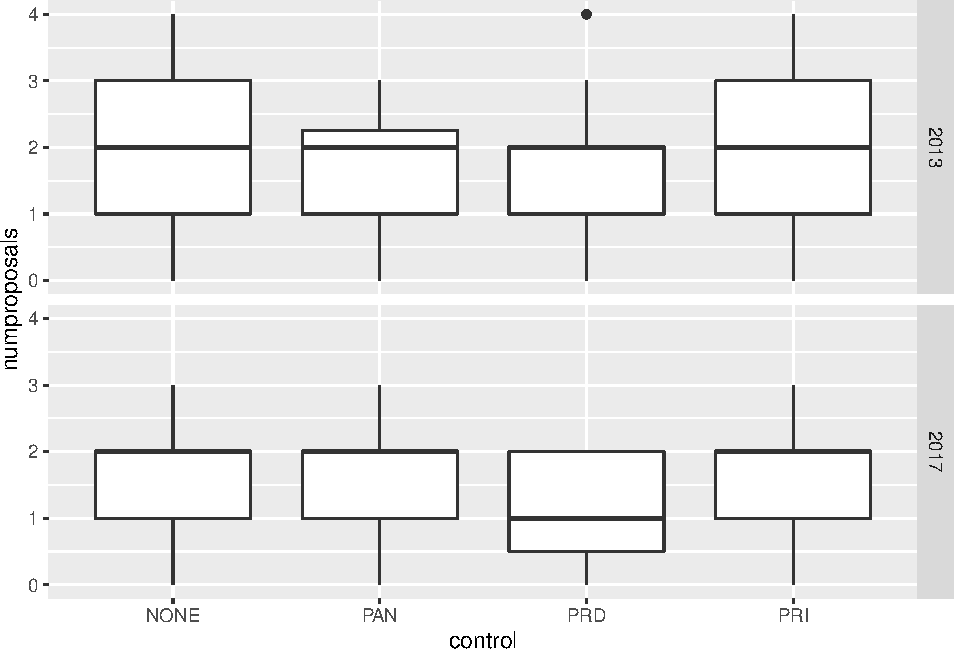
\includegraphics{ProposalAnalysis_files/figure-latex/unnamed-chunk-6-1.pdf}

\begin{Shaded}
\begin{Highlighting}[]
\CommentTok{# join with parties}
\NormalTok{ys.proposed }\OperatorTok\StringTok{ }\KeywordTok{left_join}\NormalTok{(parties.df)}
\end{Highlighting}
\end{Shaded}

\begin{verbatim}
## Joining, by = "actor"
\end{verbatim}

\begin{verbatim}
## Warning: Column `actor` joining character vector and factor, coercing into
## character vector
\end{verbatim}

\begin{verbatim}
## left_join: added one column (partytype)
\end{verbatim}

\begin{verbatim}
## Warning: Column `actor` joining character vector and factor, coercing into
## character vector
\end{verbatim}

\begin{verbatim}
## Warning: Column `actor` joining factor and character vector, coercing into
## character vector
\end{verbatim}

\begin{verbatim}
##            > rows only in x     0
\end{verbatim}

\begin{verbatim}
##            > rows only in y  (  0)
\end{verbatim}

\begin{verbatim}
##            > matched rows     737
\end{verbatim}

\begin{verbatim}
##            >                 =====
\end{verbatim}

\begin{verbatim}
##            > rows total       737
\end{verbatim}

Strategic Position Categorization

A party in a ``strong'' position political position in the state, then
they are more likely to propose than a party with a less ``strong''
position.

The decision is a function of several variables such as: party controls
the state during the redistricting year, if the party has been the sole
ruler over from 1990-2013/17, and if they have ruled a majority of that
timer period, if they have ruled at least once during that time period.

The variables used in the decision tree embody levels of competition in
each state. A state controlled by a single party during the period has
low levels of political competition, for example. A state with a party
which has not won a majority of elections but has won at least once has
some degree of power in a competitive state (there are at least two
parties competing), as another example. The former has a better
``strategic position'' than the latter.

The ``Strategic Positions'' are defined as follows: 1. Party a) Controls
during redistricting year b) has controlled state in all previous
observed periods

\begin{enumerate}
\def\labelenumi{\arabic{enumi}.}
\setcounter{enumi}{1}
\item
  Party a) Controls during redistricting year b) has NOT controlled
  state in all previously observed periods
\item
  Party a) DOES NOT control during the redistricting year b) has NOT
  controlled state in all previously observed periods c) has won a
  MAJORITY of previous elections in observed time period
\item
  Party a) DOES NOT control during the redistricting year b) has NOT
  controlled state in all previously observed periods c) has won a
  MINORITY of previous elections in observed time period
\item
  Party a) DOES NOT control during the redistricting year b) has NOT
  controlled state in all previously observed periods c) has won NONE of
  the previous elections during the time period
\item
  Party a) DOES NOT control during the redistricting year b) has NOT
  controlled state in all previously observed periods c) has won NONE of
  the previous elections during the time period d) another party has won
  ALL previous elections
\end{enumerate}

\begin{Shaded}
\begin{Highlighting}[]
\NormalTok{ys.proposed }\OperatorTok\StringTok{ }\KeywordTok{rowwise}\NormalTok{() }\OperatorTok\StringTok{ }\KeywordTok{mutate}\NormalTok{(}
    \DataTypeTok{PartyStratPos =} \KeywordTok{case_when}\NormalTok{(}
\NormalTok{      didControl }\OperatorTok{==}\StringTok{ }\OtherTok{TRUE}     \OperatorTok{~}\StringTok{ }\DecValTok{1}\NormalTok{, }\CommentTok{# in sole control entire period}
\NormalTok{      didRule }\OperatorTok{==}\StringTok{ }\OtherTok{TRUE}        \OperatorTok{~}\StringTok{ }\DecValTok{2}\NormalTok{, }\CommentTok{# NOT in sole control, but won last election}
\NormalTok{      actor }\OperatorTok{==}\StringTok{ }\NormalTok{primary       }\OperatorTok{~}\StringTok{ }\DecValTok{3}\NormalTok{, }\CommentTok{# NOT win last election, but won most elections}
\NormalTok{      didWinever }\OperatorTok{==}\StringTok{ }\OtherTok{TRUE}     \OperatorTok{~}\StringTok{ }\DecValTok{4}\NormalTok{, }\CommentTok{# NOT won most, but won at least one}
\NormalTok{      singlecontrol }\OperatorTok{==}\StringTok{ }\OtherTok{FALSE} \OperatorTok{~}\StringTok{ }\DecValTok{5}\NormalTok{, }\CommentTok{# NOT won ever,  but single party does not control}
      \OtherTok{TRUE} \OperatorTok{~}\StringTok{ }\DecValTok{6} \CommentTok{# Out party in noncompetitive state  - different party always in control}
\NormalTok{    )}
\NormalTok{  )}
\end{Highlighting}
\end{Shaded}

\begin{verbatim}
## mutate: new variable 'PartyStratPos' with 6 unique values and 0% NA
\end{verbatim}

\begin{Shaded}
\begin{Highlighting}[]
\KeywordTok{table}\NormalTok{(ys.proposed}\OperatorTok{$}\NormalTok{PartyStratPos)}
\end{Highlighting}
\end{Shaded}

\begin{verbatim}
## 
##   1   2   3   4   5   6 
##  33  31  22  14 287 350
\end{verbatim}

\begin{Shaded}
\begin{Highlighting}[]
\NormalTok{check.df <-}\StringTok{ }\NormalTok{ys.proposed }\OperatorTok\StringTok{ }\KeywordTok{filter}\NormalTok{(PartyStratPos }\OperatorTok{==}\StringTok{ }\DecValTok{6}\NormalTok{)}
\end{Highlighting}
\end{Shaded}

\begin{verbatim}
## filter: removed 387 rows (53%), 350 rows remaining
\end{verbatim}

\begin{Shaded}
\begin{Highlighting}[]
\KeywordTok{table}\NormalTok{(check.df}\OperatorTok{$}\NormalTok{edon)}
\end{Highlighting}
\end{Shaded}

\begin{verbatim}
## 
##  2  3  4  6  7  8  9 10 11 13 14 15 20 21 23 25 27 28 30 32 
## 21 11 21 21 21 21 21 21 21 21 11 21 11 11 21 11 11 21 21 11
\end{verbatim}

\begin{Shaded}
\begin{Highlighting}[]
\CommentTok{# now compute for coalitions}
\NormalTok{coalitions.df <-}\StringTok{ }\KeywordTok{read_excel}\NormalTok{(}\StringTok{"Coaltion Data State Level 2010-2016 (Coalitions and Parties).xlsx"}\NormalTok{)}
\NormalTok{coalitions.df  }\OperatorTok\StringTok{ }\KeywordTok{rowwise}\NormalTok{()   }\OperatorTok\StringTok{ }\KeywordTok{filter}\NormalTok{(}\KeywordTok{grepl}\NormalTok{(}\StringTok{'-'}\NormalTok{,actor)) }\OperatorTok\StringTok{ }\KeywordTok{mutate}\NormalTok{(}\DataTypeTok{coalition=}\NormalTok{actor)  }\OperatorTok\StringTok{ }\KeywordTok{separate_rows}\NormalTok{(actor,}\DataTypeTok{sep=}\StringTok{'-'}\NormalTok{)}
\end{Highlighting}
\end{Shaded}

\begin{verbatim}
## filter: removed 229 rows (68%), 110 rows remaining
\end{verbatim}

\begin{verbatim}
## mutate: new variable 'coalition' with 27 unique values and 0% NA
\end{verbatim}

\begin{Shaded}
\begin{Highlighting}[]
\NormalTok{coalitions.df }\OperatorTok\StringTok{ }\KeywordTok{left_join}\NormalTok{(}\KeywordTok{select}\NormalTok{(ys.proposed,}\KeywordTok{c}\NormalTok{(}\StringTok{"actor"}\NormalTok{,}\StringTok{"edon"}\NormalTok{,}\StringTok{"year"}\NormalTok{,}\StringTok{"PartyStratPos"}\NormalTok{))) }\OperatorTok\StringTok{ }\KeywordTok{group_by}\NormalTok{(edon,year,coalition) }\OperatorTok\StringTok{ }\KeywordTok{mutate}\NormalTok{(}\DataTypeTok{CoalitionStratPos=}\KeywordTok{min}\NormalTok{(PartyStratPos)) }\OperatorTok\StringTok{ }\KeywordTok{select}\NormalTok{(}\OperatorTok{-}\NormalTok{PartyStratPos)}
\end{Highlighting}
\end{Shaded}

\begin{verbatim}
## select: dropped 18 variables (numproposals, partylist, partyseq, partytab, singlecontrol, …)
\end{verbatim}

\begin{verbatim}
## Joining, by = c("edon", "year", "actor")
\end{verbatim}

\begin{verbatim}
## left_join: added one column (PartyStratPos)
\end{verbatim}

\begin{verbatim}
##            > rows only in x     0
\end{verbatim}

\begin{verbatim}
##            > rows only in y  (461)
\end{verbatim}

\begin{verbatim}
##            > matched rows     287
\end{verbatim}

\begin{verbatim}
##            >                 =====
\end{verbatim}

\begin{verbatim}
##            > rows total       287
\end{verbatim}

\begin{verbatim}
## group_by: 3 grouping variables (edon, year, coalition)
\end{verbatim}

\begin{verbatim}
## mutate (grouped): new variable 'CoalitionStratPos' with 6 unique values and 0% NA
\end{verbatim}

\begin{verbatim}
## select: dropped one variable (PartyStratPos)
\end{verbatim}

\begin{Shaded}
\begin{Highlighting}[]
\NormalTok{ys.proposed }\OperatorTok\StringTok{ }\KeywordTok{left_join}\NormalTok{(coalitions.df,}\DataTypeTok{by=}\KeywordTok{c}\NormalTok{(}\StringTok{"actor"}\NormalTok{,}\StringTok{"edon"}\NormalTok{,}\StringTok{"year"}\NormalTok{))}
\end{Highlighting}
\end{Shaded}

\begin{verbatim}
## left_join: added 5 columns (state, extension, competitiveness, coalition, CoalitionStratPos)
\end{verbatim}

\begin{verbatim}
##            > rows only in x   461
\end{verbatim}

\begin{verbatim}
##            > rows only in y  (  0)
\end{verbatim}

\begin{verbatim}
##            > matched rows     287    (includes duplicates)
\end{verbatim}

\begin{verbatim}
##            >                 =====
\end{verbatim}

\begin{verbatim}
##            > rows total       748
\end{verbatim}

\begin{Shaded}
\begin{Highlighting}[]
\NormalTok{ys.proposed }\OperatorTok\StringTok{ }\KeywordTok{mutate}\NormalTok{(}\DataTypeTok{StratPos=}\KeywordTok{if_else}\NormalTok{(}\KeywordTok{is.na}\NormalTok{(CoalitionStratPos),PartyStratPos,CoalitionStratPos))}
\end{Highlighting}
\end{Shaded}

\begin{verbatim}
## mutate: new variable 'StratPos' with 6 unique values and 0% NA
\end{verbatim}

\begin{Shaded}
\begin{Highlighting}[]
\CommentTok{#Check the categories}
\CommentTok{#Exhaustive and mutually exclusive, like we want.}

\CommentTok{#check pattern of proposal entry}
\NormalTok{xtab.result <-}\StringTok{ }\NormalTok{ys.proposed }\OperatorTok\StringTok{ }\KeywordTok{filter}\NormalTok{(partytype}\OperatorTok{==}\StringTok{"minor"} \OperatorTok{||}\StringTok{ }\NormalTok{partytype}\OperatorTok{==}\StringTok{"major"}\NormalTok{) }\OperatorTok\StringTok{ }\KeywordTok{xtabs}\NormalTok{(}\OperatorTok{~}\NormalTok{partytype}\OperatorTok{+}\NormalTok{year}\OperatorTok{+}\NormalTok{didPropose}\OperatorTok{+}\NormalTok{StratPos,.,}\DataTypeTok{drop.unused.levels =} \OtherTok{TRUE}\NormalTok{)}
\end{Highlighting}
\end{Shaded}

\begin{verbatim}
## filter: removed 225 rows (30%), 523 rows remaining
\end{verbatim}

\begin{Shaded}
\begin{Highlighting}[]
\KeywordTok{ftable}\NormalTok{(xtab.result)}
\end{Highlighting}
\end{Shaded}

\begin{verbatim}
##                           StratPos  1  2  3  4  5  6
## partytype year didPropose                           
## major     2013 FALSE                0  0  1  1  1  0
##                TRUE                25 13  7  4 10 37
##           2017 FALSE                0  0  2  0  0  1
##                TRUE                13 20 14  8 15 25
## minor     2013 FALSE                3  1  1  0  5  5
##                TRUE                27 16  2  3 21 45
##           2017 FALSE                2  0  0  1  9  7
##                TRUE                19 28  8  5 68 50
\end{verbatim}

\begin{Shaded}
\begin{Highlighting}[]
\CommentTok{#but we really want }
 
\CommentTok{#CLM model first}
\NormalTok{clm.mod <-}\StringTok{ }\NormalTok{ys.proposed }\OperatorTok\StringTok{ }\KeywordTok{filter}\NormalTok{(partytype}\OperatorTok{==}\StringTok{"major"}\NormalTok{) }\OperatorTok\StringTok{ }\KeywordTok{clm}\NormalTok{(}\KeywordTok{as.ordered}\NormalTok{(didPropose)}\OperatorTok{~}\KeywordTok{as.ordered}\NormalTok{(StratPos), }\DataTypeTok{data=}\NormalTok{.)}
\end{Highlighting}
\end{Shaded}

\begin{verbatim}
## filter: removed 551 rows (74%), 197 rows remaining
\end{verbatim}

\begin{verbatim}
## Warning: (1) Hessian is numerically singular: parameters are not uniquely determined 
## In addition: Absolute convergence criterion was met, but relative criterion was not met
\end{verbatim}

\begin{Shaded}
\begin{Highlighting}[]
\KeywordTok{summary}\NormalTok{(clm.mod)}
\end{Highlighting}
\end{Shaded}

\begin{verbatim}
## formula: as.ordered(didPropose) ~ as.ordered(StratPos)
## data:    .
## 
##  link  threshold nobs logLik AIC   niter max.grad cond.H 
##  logit flexible  197  -21.94 55.88 21(0) 5.95e-09 2.2e+09
## 
## Coefficients:
##                        Estimate Std. Error z value Pr(>|z|)
## as.ordered(StratPos).L  -18.501         NA      NA       NA
## as.ordered(StratPos).Q   10.093         NA      NA       NA
## as.ordered(StratPos).C    3.157         NA      NA       NA
## as.ordered(StratPos)^4   -8.140         NA      NA       NA
## as.ordered(StratPos)^5    5.432         NA      NA       NA
## 
## Threshold coefficients:
##            Estimate Std. Error z value
## FALSE|TRUE   -9.697         NA      NA
\end{verbatim}

\begin{Shaded}
\begin{Highlighting}[]
\CommentTok{#example of ordinal model only, seems to have numerical problems}
\NormalTok{model.results <-}\StringTok{ }\NormalTok{ys.proposed }\OperatorTok\StringTok{ }\KeywordTok{filter}\NormalTok{(partytype}\OperatorTok{==}\StringTok{"major"}\NormalTok{) }\OperatorTok\StringTok{ }\KeywordTok{clmm}\NormalTok{(}\KeywordTok{as.ordered}\NormalTok{(didPropose)}\OperatorTok{~}\KeywordTok{as.ordered}\NormalTok{(StratPos)}\OperatorTok{+}\NormalTok{(}\DecValTok{1}\OperatorTok{|}\NormalTok{actor),.)}
\end{Highlighting}
\end{Shaded}

\begin{verbatim}
## filter: removed 551 rows (74%), 197 rows remaining
\end{verbatim}

\begin{verbatim}
## Warning: (1) Hessian is numerically singular: parameters are not uniquely determined 
## In addition: Absolute convergence criterion was met, but relative criterion was not met
\end{verbatim}

\begin{Shaded}
\begin{Highlighting}[]
\KeywordTok{summary}\NormalTok{(model.results)}
\end{Highlighting}
\end{Shaded}

\begin{verbatim}
## Warning in summary.clmm(model.results): Variance-covariance matrix of the
## parameters is not defined
\end{verbatim}

\begin{verbatim}
## Cumulative Link Mixed Model fitted with the Laplace approximation
## 
## formula: as.ordered(didPropose) ~ as.ordered(StratPos) + (1 | actor)
## data:    .
## 
##  link  threshold nobs logLik AIC   niter    max.grad cond.H
##  logit flexible  197  -21.69 57.38 204(615) 2.60e-06 NaN   
## 
## Random effects:
##  Groups Name        Variance Std.Dev.
##  actor  (Intercept) 0.5035   0.7096  
## Number of groups:  actor 3 
## 
## Coefficients:
##                        Estimate Std. Error z value Pr(>|z|)
## as.ordered(StratPos).L  -18.256         NA      NA       NA
## as.ordered(StratPos).Q   10.270         NA      NA       NA
## as.ordered(StratPos).C    2.954         NA      NA       NA
## as.ordered(StratPos)^4   -8.446         NA      NA       NA
## as.ordered(StratPos)^5    5.451         NA      NA       NA
## 
## Threshold coefficients:
##            Estimate Std. Error z value
## FALSE|TRUE     -9.9         NA      NA
\end{verbatim}

\begin{Shaded}
\begin{Highlighting}[]
\CommentTok{#Pretty much exact same output from slightly different variations of the cumulative model. I do not think using "polr()" or a monotonic model would be appropriate for our data. Neither accounts for ordinal independent variables and the "ordinal" package can handle ordincal dependent variables if we want to try to predict partytype or StratPos using the data on hand.}
\end{Highlighting}
\end{Shaded}

\#H.1.1.1.a \#Comparing the decision of the ruling party to formulate a
counterproposal to other parties in that same state --\textgreater{}
Requires a dummy capturing if the state had single party dominance
(single\_pty\_dom\_00\_17:True) --\textgreater{} In those states where
the condition is met --\textgreater{} the ruling party is more likely to
formulate a counterporposal than each opposition party in that same
state.

\#Method: Difference of means test: H1: mean of ENTRY for the Ruling
Party in a state with single party dominance \textgreater{} mean of
ENTRY for each opposition party in that same state; H0: mean of ENTRY
for the Ruling Party in a state with single party dominance \textless=
mean of ENTRY for (each) opposition parties in that same state.

\begin{Shaded}
\begin{Highlighting}[]
\KeywordTok{require}\NormalTok{(broom)}
\end{Highlighting}
\end{Shaded}

\begin{verbatim}
## Loading required package: broom
\end{verbatim}

\begin{Shaded}
\begin{Highlighting}[]
\KeywordTok{require}\NormalTok{(GGally)}
\end{Highlighting}
\end{Shaded}

\begin{verbatim}
## Loading required package: GGally
\end{verbatim}

\begin{verbatim}
## Registered S3 method overwritten by 'GGally':
##   method from   
##   +.gg   ggplot2
\end{verbatim}

\begin{verbatim}
## 
## Attaching package: 'GGally'
\end{verbatim}

\begin{verbatim}
## The following object is masked from 'package:dplyr':
## 
##     nasa
\end{verbatim}

\begin{Shaded}
\begin{Highlighting}[]
\NormalTok{tabfit <-}\StringTok{ }\NormalTok{ys.proposed }\OperatorTok\StringTok{ }\KeywordTok{xtabs}\NormalTok{(}\OperatorTok{~}\NormalTok{didPropose}\OperatorTok{+}\NormalTok{didControl}\OperatorTok{+}\NormalTok{year,}\DataTypeTok{data=}\NormalTok{.)}
\KeywordTok{print}\NormalTok{(tabfit)}
\end{Highlighting}
\end{Shaded}

\begin{verbatim}
## , , year = 2013
## 
##           didControl
## didPropose FALSE TRUE
##      FALSE    75    0
##      TRUE    291   22
## 
## , , year = 2017
## 
##           didControl
## didPropose FALSE TRUE
##      FALSE    23    0
##      TRUE    324   13
\end{verbatim}

\begin{Shaded}
\begin{Highlighting}[]
\KeywordTok{ftable}\NormalTok{(tabfit)}
\end{Highlighting}
\end{Shaded}

\begin{verbatim}
##                       year 2013 2017
## didPropose didControl               
## FALSE      FALSE             75   23
##            TRUE               0    0
## TRUE       FALSE            291  324
##            TRUE              22   13
\end{verbatim}

\begin{Shaded}
\begin{Highlighting}[]
\NormalTok{ys.proposed }\OperatorTok\StringTok{ }\KeywordTok{ggplot}\NormalTok{(}\KeywordTok{aes}\NormalTok{(didControl,didPropose))}\OperatorTok{+}\KeywordTok{geom_col}\NormalTok{()}\OperatorTok{+}\KeywordTok{facet_grid}\NormalTok{(}\DataTypeTok{rows=}\KeywordTok{vars}\NormalTok{(year))}
\end{Highlighting}
\end{Shaded}

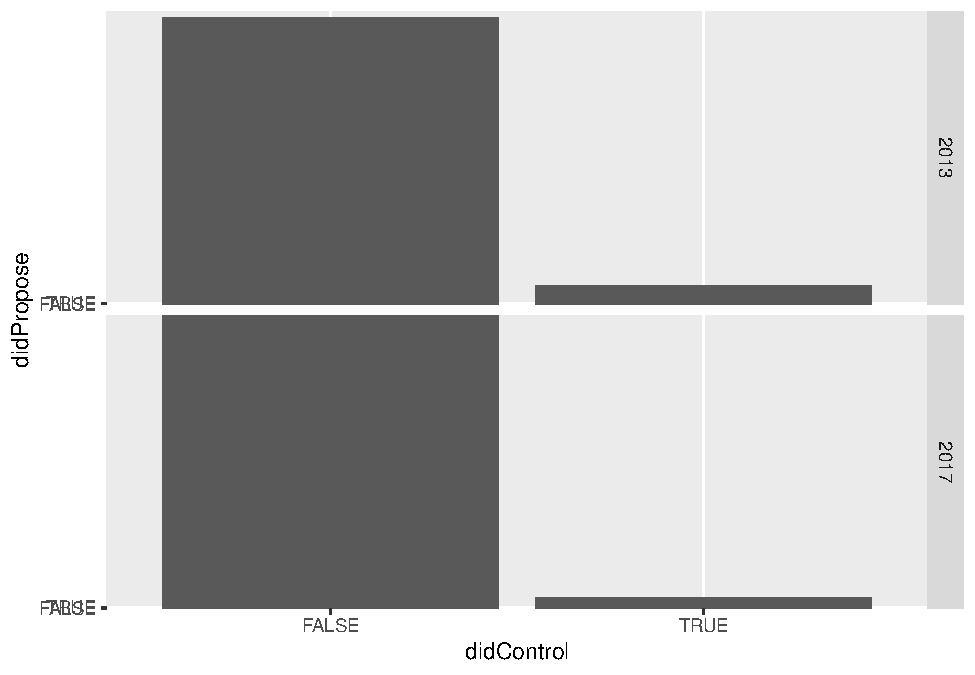
\includegraphics{ProposalAnalysis_files/figure-latex/unnamed-chunk-8-1.pdf}

\begin{Shaded}
\begin{Highlighting}[]
\NormalTok{glmfit <-}\StringTok{ }\NormalTok{ys.proposed }\OperatorTok\StringTok{ }\KeywordTok{glm}\NormalTok{(didPropose}\OperatorTok{~}\NormalTok{didControl}\OperatorTok{+}\NormalTok{year,}\DataTypeTok{data=}\NormalTok{.,}\DataTypeTok{family=}\KeywordTok{binomial}\NormalTok{())}
\KeywordTok{summary}\NormalTok{(glmfit)}
\end{Highlighting}
\end{Shaded}

\begin{verbatim}
## 
## Call:
## glm(formula = didPropose ~ didControl + year, family = binomial(), 
##     data = .)
## 
## Deviance Residuals: 
##     Min       1Q   Median       3Q      Max  
## -2.3297   0.3704   0.3704   0.6772   0.6772  
## 
## Coefficients:
##                  Estimate Std. Error z value Pr(>|z|)    
## (Intercept)    -647.54183  126.71626  -5.110 3.22e-07 ***
## didControlTRUE   15.84098  650.33608   0.024    0.981    
## year              0.32235    0.06292   5.124 3.00e-07 ***
## ---
## Signif. codes:  0 '***' 0.001 '**' 0.01 '*' 0.05 '.' 0.1 ' ' 1
## 
## (Dispersion parameter for binomial family taken to be 1)
## 
##     Null deviance: 580.92  on 747  degrees of freedom
## Residual deviance: 540.51  on 745  degrees of freedom
## AIC: 546.51
## 
## Number of Fisher Scoring iterations: 16
\end{verbatim}

\begin{Shaded}
\begin{Highlighting}[]
\KeywordTok{augment}\NormalTok{(glmfit) }\OperatorTok\StringTok{ }\KeywordTok{ggplot}\NormalTok{(}\KeywordTok{aes}\NormalTok{(didPropose,.fitted))}\OperatorTok{+}\KeywordTok{geom_jitter}\NormalTok{()}\OperatorTok{+}\KeywordTok{facet_grid}\NormalTok{(}\DataTypeTok{rows=}\KeywordTok{vars}\NormalTok{(didControl))}
\end{Highlighting}
\end{Shaded}

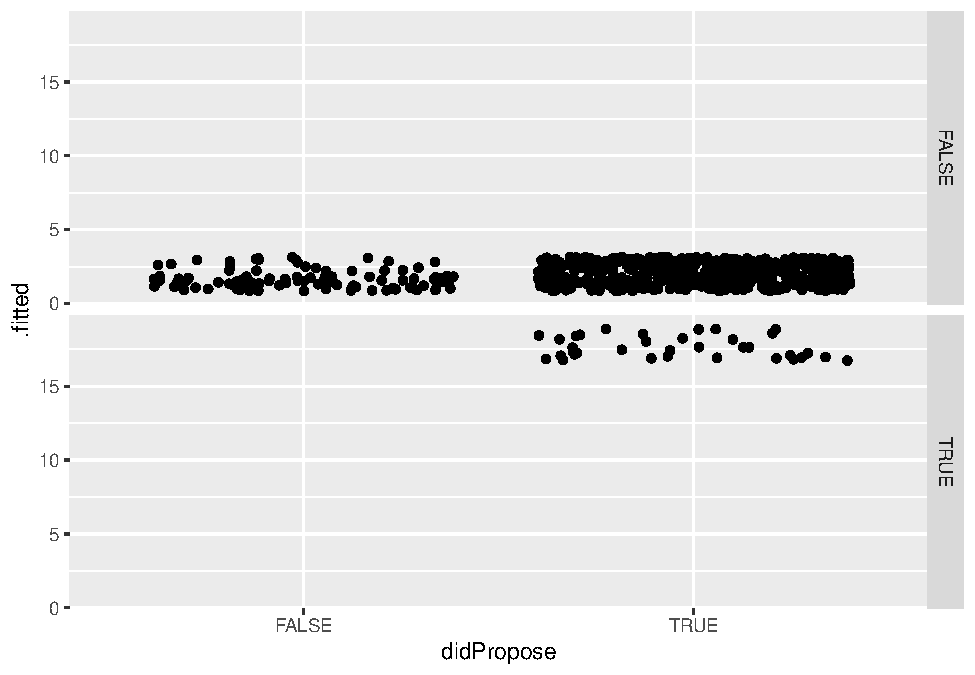
\includegraphics{ProposalAnalysis_files/figure-latex/unnamed-chunk-8-2.pdf}

\begin{Shaded}
\begin{Highlighting}[]
\KeywordTok{ggcoef}\NormalTok{(glmfit)}
\end{Highlighting}
\end{Shaded}

\begin{verbatim}
## Warning: glm.fit: fitted probabilities numerically 0 or 1 occurred

## Warning: glm.fit: fitted probabilities numerically 0 or 1 occurred

## Warning: glm.fit: fitted probabilities numerically 0 or 1 occurred

## Warning: glm.fit: fitted probabilities numerically 0 or 1 occurred

## Warning: glm.fit: fitted probabilities numerically 0 or 1 occurred

## Warning: glm.fit: fitted probabilities numerically 0 or 1 occurred

## Warning: glm.fit: fitted probabilities numerically 0 or 1 occurred

## Warning: glm.fit: fitted probabilities numerically 0 or 1 occurred

## Warning: glm.fit: fitted probabilities numerically 0 or 1 occurred

## Warning: glm.fit: fitted probabilities numerically 0 or 1 occurred

## Warning: glm.fit: fitted probabilities numerically 0 or 1 occurred

## Warning: glm.fit: fitted probabilities numerically 0 or 1 occurred

## Warning: glm.fit: fitted probabilities numerically 0 or 1 occurred

## Warning: glm.fit: fitted probabilities numerically 0 or 1 occurred

## Warning: glm.fit: fitted probabilities numerically 0 or 1 occurred

## Warning: glm.fit: fitted probabilities numerically 0 or 1 occurred

## Warning: glm.fit: fitted probabilities numerically 0 or 1 occurred

## Warning: glm.fit: fitted probabilities numerically 0 or 1 occurred

## Warning: glm.fit: fitted probabilities numerically 0 or 1 occurred

## Warning: glm.fit: fitted probabilities numerically 0 or 1 occurred
\end{verbatim}

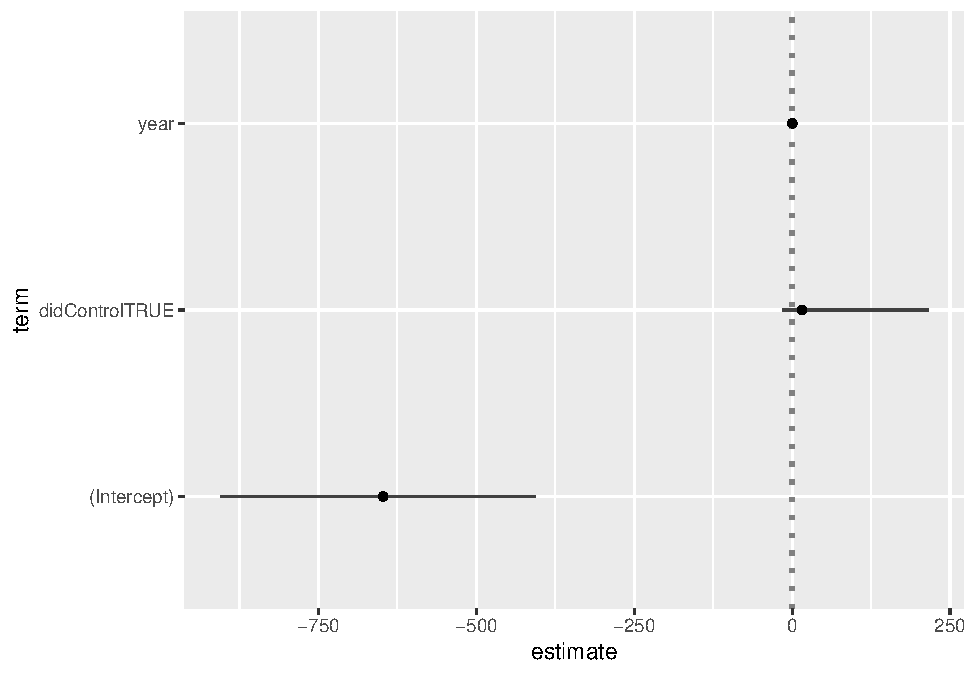
\includegraphics{ProposalAnalysis_files/figure-latex/unnamed-chunk-8-3.pdf}

Build Alternation Data Frame Variables relate to the ``competitiveness''
of the state (i.e.~more alternation = higher levels of competition)

\hypertarget{needs-to-be-reworked-for-ys.proposed-as-df}{%
\section{NEEDS TO BE REWORKED for ys.proposed as
df}\label{needs-to-be-reworked-for-ys.proposed-as-df}}

Some visualizations

\begin{Shaded}
\begin{Highlighting}[]
\NormalTok{ys.proposed }\OperatorTok\StringTok{ }\KeywordTok{ggplot}\NormalTok{(}\KeywordTok{aes}\NormalTok{(StratPos)) }\OperatorTok{+}\StringTok{ }\KeywordTok{geom_histogram}\NormalTok{() }\OperatorTok{+}\KeywordTok{facet_wrap}\NormalTok{(}\OperatorTok{~}\NormalTok{year)}
\end{Highlighting}
\end{Shaded}

\begin{verbatim}
## `stat_bin()` using `bins = 30`. Pick better value with `binwidth`.
\end{verbatim}

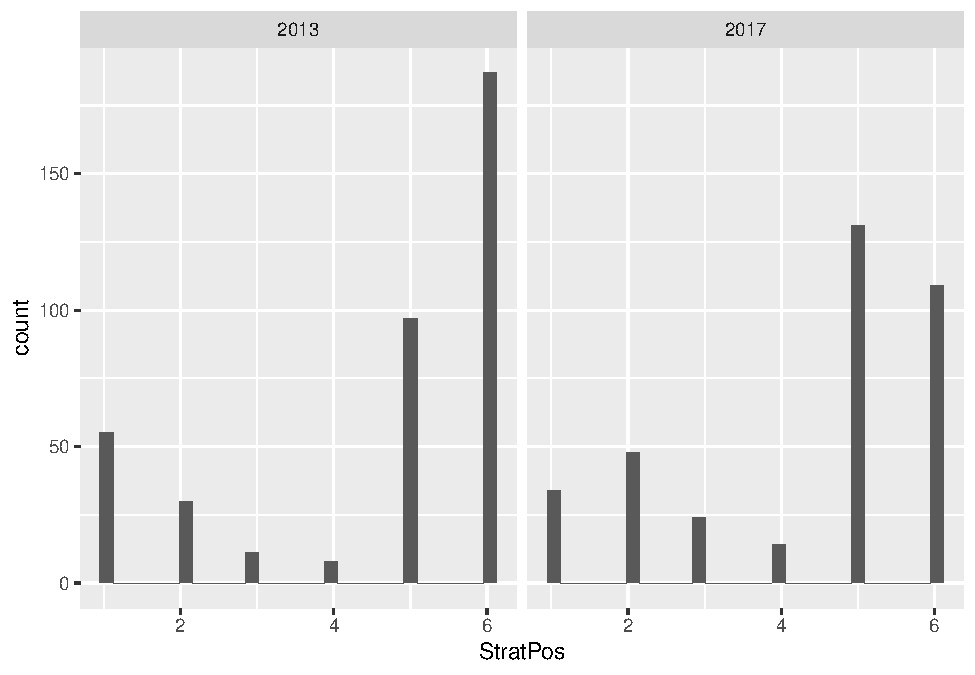
\includegraphics{ProposalAnalysis_files/figure-latex/unnamed-chunk-9-1.pdf}

\begin{Shaded}
\begin{Highlighting}[]
\NormalTok{ys.proposed }\OperatorTok\StringTok{ }\KeywordTok{filter}\NormalTok{(partytype }\OperatorTok{==}\StringTok{ "major"} \OperatorTok{|}\StringTok{ }\NormalTok{partytype }\OperatorTok{==}\StringTok{ "minor"} \OperatorTok{&}\StringTok{ }\NormalTok{year }\OperatorTok{==}\StringTok{ }\DecValTok{2013}\NormalTok{) }\OperatorTok\StringTok{ }\KeywordTok{ggplot}\NormalTok{(}\KeywordTok{aes}\NormalTok{(StratPos)) }\OperatorTok{+}\StringTok{ }\KeywordTok{geom_histogram}\NormalTok{() }\OperatorTok{+}\StringTok{ }\KeywordTok{facet_wrap}\NormalTok{(}\OperatorTok{~}\NormalTok{actor)}
\end{Highlighting}
\end{Shaded}

\begin{verbatim}
## filter: removed 422 rows (56%), 326 rows remaining
## `stat_bin()` using `bins = 30`. Pick better value with `binwidth`.
\end{verbatim}

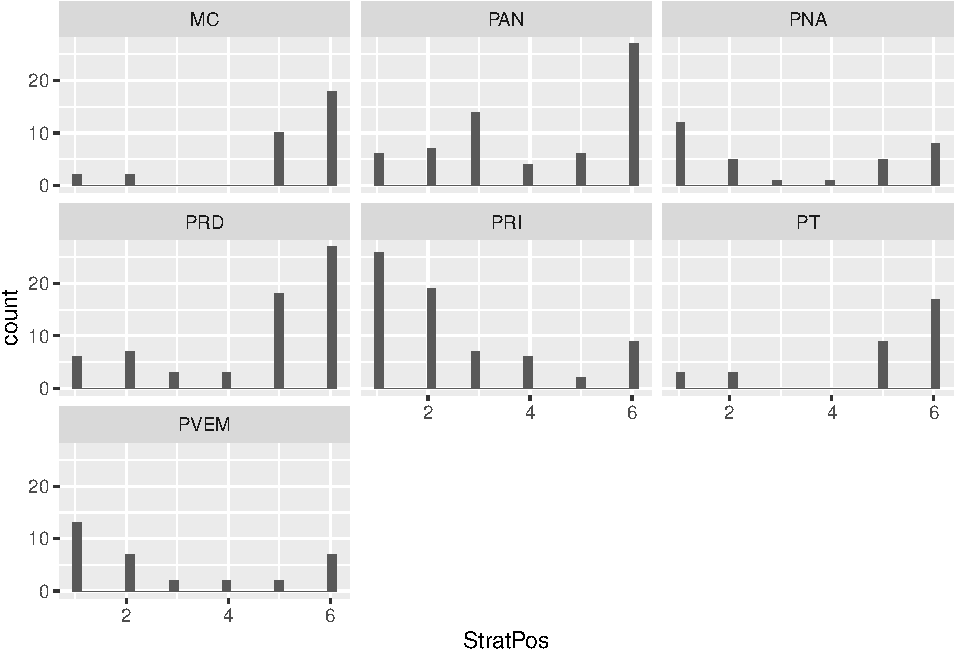
\includegraphics{ProposalAnalysis_files/figure-latex/unnamed-chunk-9-2.pdf}

\begin{Shaded}
\begin{Highlighting}[]
\NormalTok{ys.proposed }\OperatorTok\StringTok{ }\KeywordTok{filter}\NormalTok{(partytype }\OperatorTok{==}\StringTok{ "major"} \OperatorTok{|}\StringTok{ }\NormalTok{partytype }\OperatorTok{==}\StringTok{ "minor"} \OperatorTok{&}\StringTok{ }\NormalTok{year }\OperatorTok{==}\StringTok{ }\DecValTok{2017}\NormalTok{) }\OperatorTok\StringTok{ }\KeywordTok{ggplot}\NormalTok{(}\KeywordTok{aes}\NormalTok{(StratPos)) }\OperatorTok{+}\StringTok{ }\KeywordTok{geom_histogram}\NormalTok{() }\OperatorTok{+}\StringTok{ }\KeywordTok{facet_wrap}\NormalTok{(}\OperatorTok{~}\NormalTok{actor)}
\end{Highlighting}
\end{Shaded}

\begin{verbatim}
## filter: removed 354 rows (47%), 394 rows remaining
## `stat_bin()` using `bins = 30`. Pick better value with `binwidth`.
\end{verbatim}

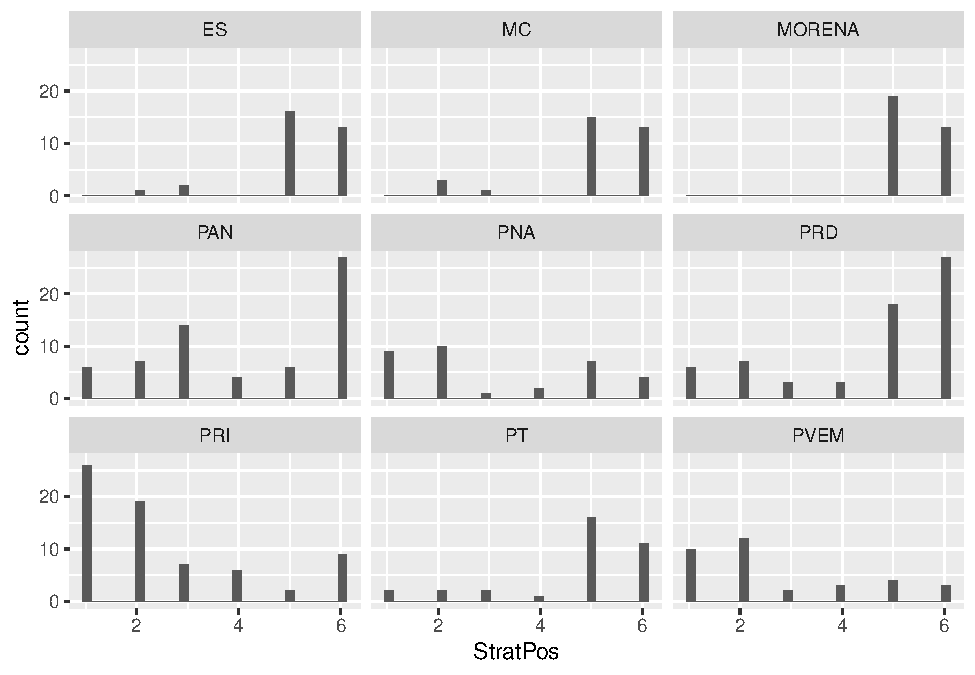
\includegraphics{ProposalAnalysis_files/figure-latex/unnamed-chunk-9-3.pdf}

\begin{Shaded}
\begin{Highlighting}[]
\NormalTok{ys.proposed }\OperatorTok\StringTok{ }\KeywordTok{filter}\NormalTok{(partytype }\OperatorTok{==}\StringTok{ "major"} \OperatorTok{|}\StringTok{ }\NormalTok{partytype }\OperatorTok{==}\StringTok{ "minor"}\NormalTok{) }\OperatorTok\StringTok{ }\KeywordTok{ggplot}\NormalTok{(}\KeywordTok{aes}\NormalTok{(StratPos)) }\OperatorTok{+}\StringTok{ }\KeywordTok{geom_histogram}\NormalTok{() }\OperatorTok{+}\StringTok{ }\KeywordTok{facet_wrap}\NormalTok{(}\OperatorTok{~}\NormalTok{partytype)}
\end{Highlighting}
\end{Shaded}

\begin{verbatim}
## filter: removed 225 rows (30%), 523 rows remaining
## `stat_bin()` using `bins = 30`. Pick better value with `binwidth`.
\end{verbatim}

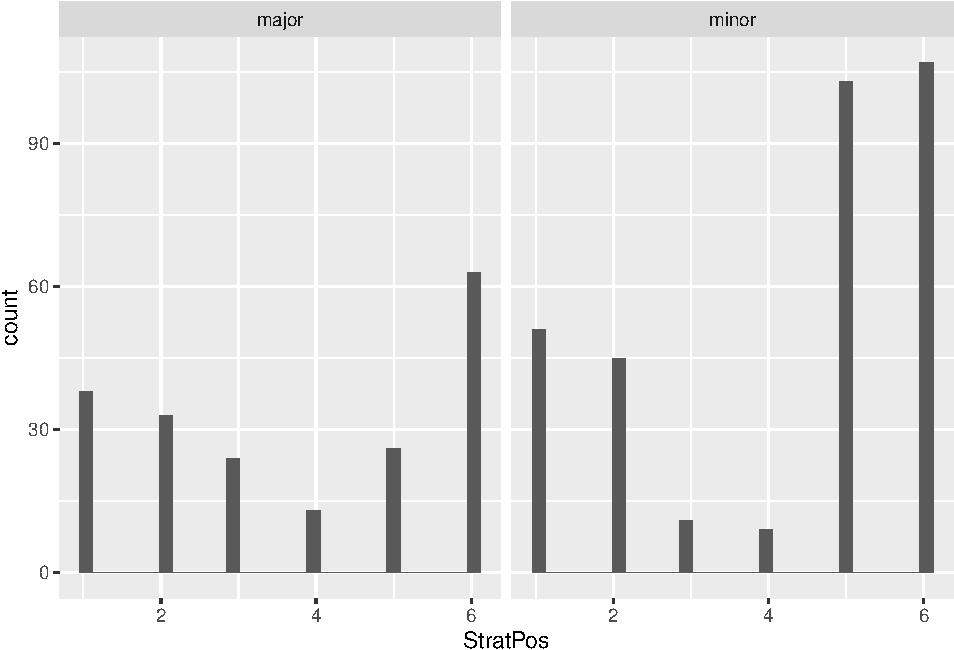
\includegraphics{ProposalAnalysis_files/figure-latex/unnamed-chunk-9-4.pdf}

\begin{Shaded}
\begin{Highlighting}[]
\NormalTok{ys.proposed }\OperatorTok\StringTok{ }\KeywordTok{ggplot}\NormalTok{(}\KeywordTok{aes}\NormalTok{(didPropose)) }\OperatorTok{+}\StringTok{ }\KeywordTok{geom_bar}\NormalTok{()}
\end{Highlighting}
\end{Shaded}

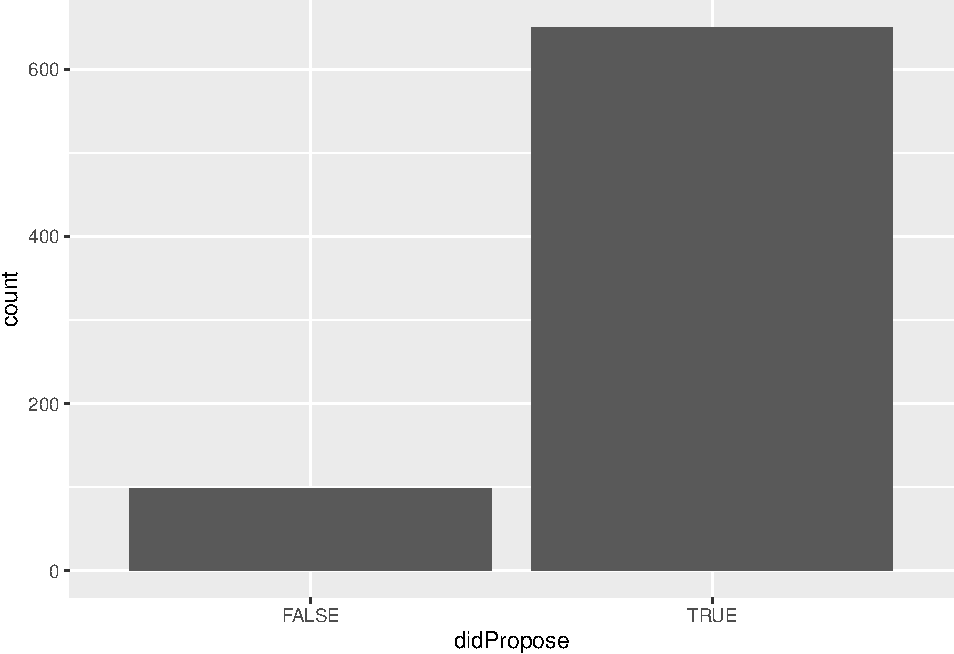
\includegraphics{ProposalAnalysis_files/figure-latex/unnamed-chunk-9-5.pdf}

\begin{Shaded}
\begin{Highlighting}[]
\NormalTok{ys.proposed }\OperatorTok\StringTok{ }\KeywordTok{ggplot}\NormalTok{(}\KeywordTok{aes}\NormalTok{(didPropose)) }\OperatorTok{+}\StringTok{ }\KeywordTok{geom_bar}\NormalTok{() }\OperatorTok{+}\StringTok{ }\KeywordTok{facet_wrap}\NormalTok{(}\OperatorTok{~}\NormalTok{partytype)}
\end{Highlighting}
\end{Shaded}

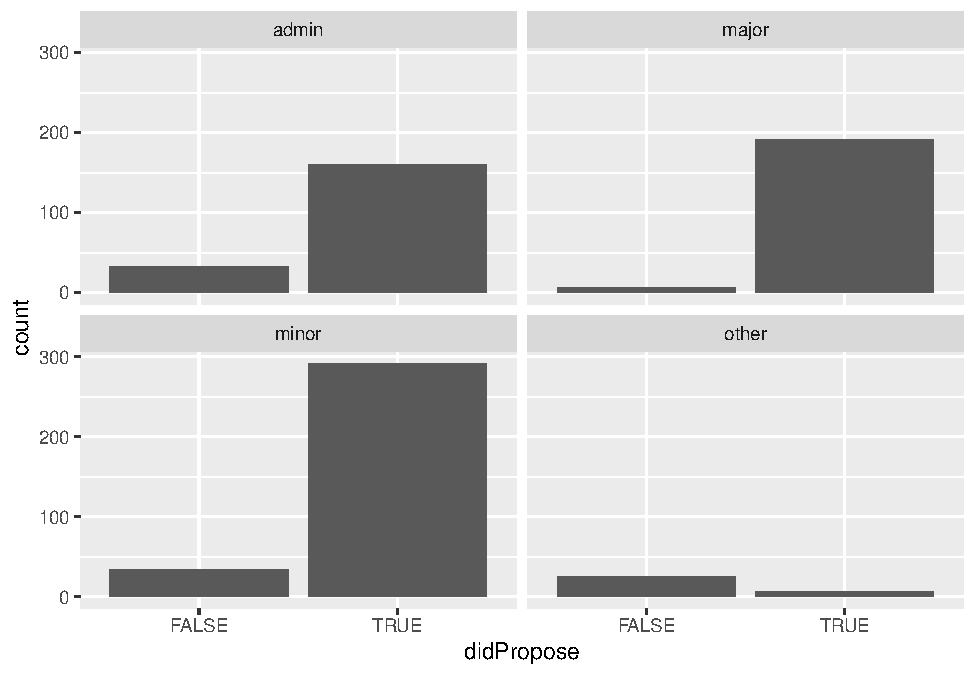
\includegraphics{ProposalAnalysis_files/figure-latex/unnamed-chunk-9-6.pdf}

\begin{Shaded}
\begin{Highlighting}[]
\NormalTok{ys.proposed }\OperatorTok\StringTok{ }\KeywordTok{ggplot}\NormalTok{(}\KeywordTok{aes}\NormalTok{(didPropose)) }\OperatorTok{+}\StringTok{ }\KeywordTok{geom_bar}\NormalTok{() }\OperatorTok{+}\StringTok{ }\KeywordTok{facet_wrap}\NormalTok{(}\OperatorTok{~}\NormalTok{StratPos)}
\end{Highlighting}
\end{Shaded}

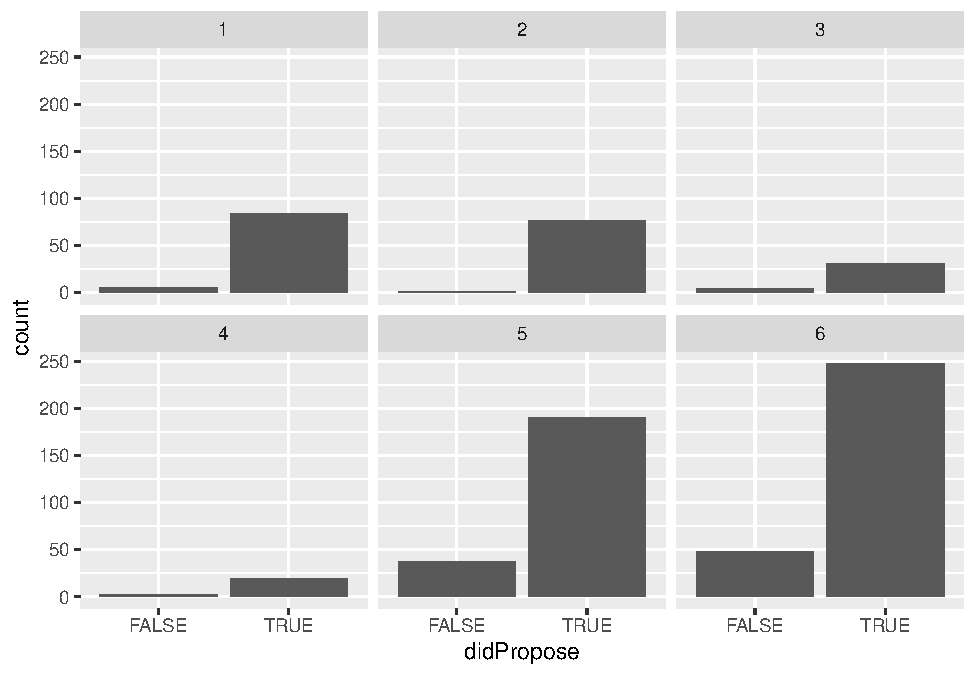
\includegraphics{ProposalAnalysis_files/figure-latex/unnamed-chunk-9-7.pdf}

Models Decision Tree

\begin{Shaded}
\begin{Highlighting}[]
\CommentTok{#Build a train/test sets}
\NormalTok{index <-}\StringTok{ }\KeywordTok{sample}\NormalTok{(}\DecValTok{1}\OperatorTok{:}\KeywordTok{nrow}\NormalTok{(ys.proposed))}
\NormalTok{ys.proposed <-}\StringTok{ }\NormalTok{ys.proposed[index,]}

\NormalTok{create_train_test <-}\StringTok{ }\ControlFlowTok{function}\NormalTok{(data, }\DataTypeTok{size=}\FloatTok{0.7}\NormalTok{, }\DataTypeTok{train=}\OtherTok{TRUE}\NormalTok{)\{}
\NormalTok{  nrow =}\StringTok{ }\KeywordTok{nrow}\NormalTok{(data)}
\NormalTok{  total_row =}\StringTok{ }\NormalTok{size}\OperatorTok{*}\NormalTok{nrow}
\NormalTok{  train_samp <-}\StringTok{ }\DecValTok{1}\OperatorTok{:}\NormalTok{total_row}
  \ControlFlowTok{if}\NormalTok{(train}\OperatorTok{==}\OtherTok{TRUE}\NormalTok{)\{}
    \KeywordTok{return}\NormalTok{(data[train_samp,])}
\NormalTok{  \}}\ControlFlowTok{else}\NormalTok{\{}
    \KeywordTok{return}\NormalTok{(data[}\OperatorTok{-}\NormalTok{train_samp,])}
\NormalTok{  \}}
\NormalTok{\}}

\NormalTok{train <-}\StringTok{ }\KeywordTok{create_train_test}\NormalTok{(ys.proposed, }\FloatTok{0.7}\NormalTok{, }\DataTypeTok{train =} \OtherTok{TRUE}\NormalTok{)}
\NormalTok{test <-}\StringTok{ }\KeywordTok{create_train_test}\NormalTok{(ys.proposed, }\FloatTok{0.7}\NormalTok{, }\DataTypeTok{train =} \OtherTok{FALSE}\NormalTok{)}
\KeywordTok{dim}\NormalTok{(train)}
\end{Highlighting}
\end{Shaded}

\begin{verbatim}
## [1] 523  28
\end{verbatim}

\begin{Shaded}
\begin{Highlighting}[]
\KeywordTok{dim}\NormalTok{(test)}
\end{Highlighting}
\end{Shaded}

\begin{verbatim}
## [1] 225  28
\end{verbatim}

\begin{Shaded}
\begin{Highlighting}[]
\KeywordTok{prop.table}\NormalTok{(}\KeywordTok{table}\NormalTok{(train}\OperatorTok{$}\NormalTok{didPropose))}
\end{Highlighting}
\end{Shaded}

\begin{verbatim}
## 
##     FALSE      TRUE 
## 0.1281071 0.8718929
\end{verbatim}

\begin{Shaded}
\begin{Highlighting}[]
\KeywordTok{prop.table}\NormalTok{(}\KeywordTok{table}\NormalTok{(test}\OperatorTok{$}\NormalTok{didPropose))}
\end{Highlighting}
\end{Shaded}

\begin{verbatim}
## 
##     FALSE      TRUE 
## 0.1377778 0.8622222
\end{verbatim}

\begin{Shaded}
\begin{Highlighting}[]
\KeywordTok{library}\NormalTok{(rpart)}
\KeywordTok{library}\NormalTok{(rpart.plot)}

\NormalTok{DT}\FloatTok{.1}\NormalTok{ <-}\StringTok{ }\KeywordTok{rpart}\NormalTok{(didPropose }\OperatorTok{~}\StringTok{ }\NormalTok{actor, }\DataTypeTok{data =}\NormalTok{ train, }\DataTypeTok{method =} \StringTok{"class"}\NormalTok{)}
\KeywordTok{rpart.plot}\NormalTok{(DT}\FloatTok{.1}\NormalTok{, }\DataTypeTok{extra=}\DecValTok{106}\NormalTok{)}
\end{Highlighting}
\end{Shaded}

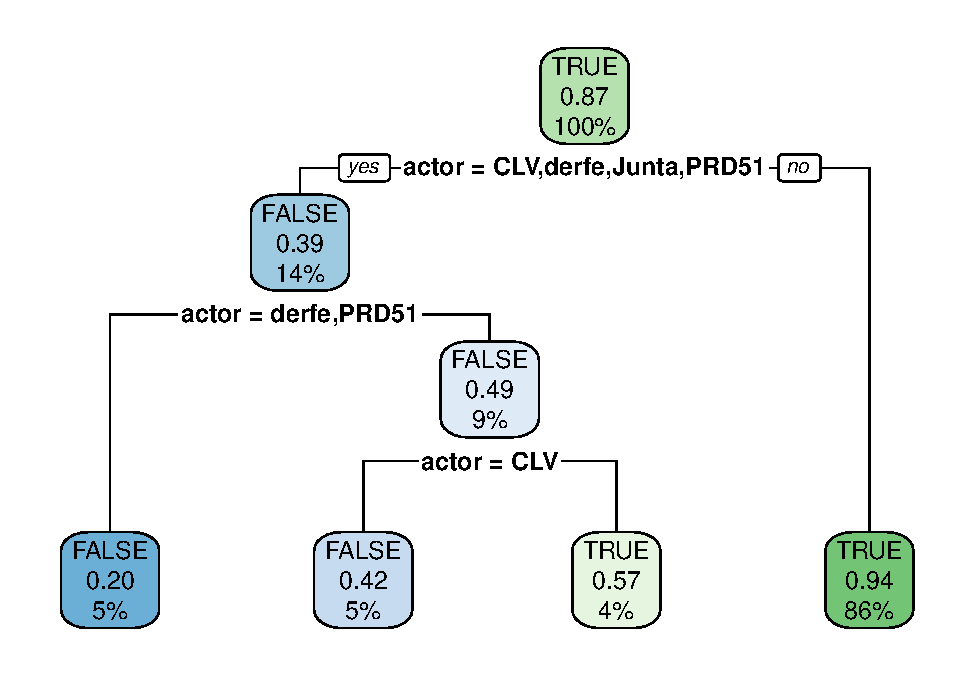
\includegraphics{ProposalAnalysis_files/figure-latex/unnamed-chunk-10-1.pdf}

\begin{Shaded}
\begin{Highlighting}[]
\CommentTok{#Its clear that since the data is unbalanced, strategic categorization is unable to beat a theoretic random draw. Rare events and/or ordinal logistic models may better reflect the actual process which we are trying to explain.}
\end{Highlighting}
\end{Shaded}

Logistic Models

\begin{Shaded}
\begin{Highlighting}[]
\CommentTok{#1. Logistic}
\NormalTok{Mod}\FloatTok{.1}\NormalTok{ <-}\StringTok{ }\NormalTok{ys.proposed }\OperatorTok\StringTok{ }\KeywordTok{filter}\NormalTok{(partytype }\OperatorTok{==}\StringTok{ "major"}\NormalTok{) }\OperatorTok\StringTok{ }\KeywordTok{glm}\NormalTok{(didPropose }\OperatorTok{~}\StringTok{ }\KeywordTok{as.factor}\NormalTok{(StratPos), }\DataTypeTok{data=}\NormalTok{., }\DataTypeTok{family =}\NormalTok{ binomial)}
\end{Highlighting}
\end{Shaded}

\begin{verbatim}
## filter: removed 551 rows (74%), 197 rows remaining
\end{verbatim}

\begin{Shaded}
\begin{Highlighting}[]
\NormalTok{Mod}\FloatTok{.2}\NormalTok{ <-}\StringTok{ }\NormalTok{ys.proposed }\OperatorTok\StringTok{ }\KeywordTok{glm}\NormalTok{(didPropose }\OperatorTok{~}\StringTok{  }\KeywordTok{as.factor}\NormalTok{(partytype), }\DataTypeTok{data=}\NormalTok{., }\DataTypeTok{family =}\NormalTok{ binomial)}

\KeywordTok{summary}\NormalTok{(Mod}\FloatTok{.1}\NormalTok{)}
\end{Highlighting}
\end{Shaded}

\begin{verbatim}
## 
## Call:
## glm(formula = didPropose ~ as.factor(StratPos), family = binomial, 
##     data = .)
## 
## Deviance Residuals: 
##      Min        1Q    Median        3Q       Max  
## -2.87859   0.00005   0.17889   0.28007   0.51678  
## 
## Coefficients:
##                        Estimate Std. Error z value Pr(>|z|)
## (Intercept)           2.057e+01  2.876e+03   0.007    0.994
## as.factor(StratPos)2 -8.413e-09  4.219e+03   0.000    1.000
## as.factor(StratPos)3 -1.862e+01  2.876e+03  -0.006    0.995
## as.factor(StratPos)4 -1.808e+01  2.876e+03  -0.006    0.995
## as.factor(StratPos)5 -1.735e+01  2.876e+03  -0.006    0.995
## as.factor(StratPos)6 -1.644e+01  2.876e+03  -0.006    0.995
## 
## (Dispersion parameter for binomial family taken to be 1)
## 
##     Null deviance: 53.713  on 196  degrees of freedom
## Residual deviance: 43.883  on 191  degrees of freedom
## AIC: 55.883
## 
## Number of Fisher Scoring iterations: 19
\end{verbatim}

\begin{Shaded}
\begin{Highlighting}[]
\KeywordTok{summary}\NormalTok{(Mod}\FloatTok{.2}\NormalTok{)}
\end{Highlighting}
\end{Shaded}

\begin{verbatim}
## 
## Call:
## glm(formula = didPropose ~ as.factor(partytype), family = binomial, 
##     data = .)
## 
## Deviance Residuals: 
##     Min       1Q   Median       3Q      Max  
## -2.6425   0.2487   0.4693   0.4693   1.7435  
## 
## Coefficients:
##                           Estimate Std. Error z value Pr(>|z|)    
## (Intercept)                 1.5787     0.1912   8.257  < 2e-16 ***
## as.factor(partytype)major   1.8818     0.4566   4.122 3.76e-05 ***
## as.factor(partytype)minor   0.5717     0.2634   2.170     0.03 *  
## as.factor(partytype)other  -2.8516     0.4684  -6.088 1.14e-09 ***
## ---
## Signif. codes:  0 '***' 0.001 '**' 0.01 '*' 0.05 '.' 0.1 ' ' 1
## 
## (Dispersion parameter for binomial family taken to be 1)
## 
##     Null deviance: 580.92  on 747  degrees of freedom
## Residual deviance: 481.95  on 744  degrees of freedom
## AIC: 489.95
## 
## Number of Fisher Scoring iterations: 6
\end{verbatim}

Rare Events Model

\begin{Shaded}
\begin{Highlighting}[]
\KeywordTok{xtabs}\NormalTok{(}\OperatorTok{~}\NormalTok{ys.proposed}\OperatorTok{$}\NormalTok{didPropose)}
\end{Highlighting}
\end{Shaded}

\begin{verbatim}
## ys.proposed$didPropose
## FALSE  TRUE 
##    98   650
\end{verbatim}

\begin{Shaded}
\begin{Highlighting}[]
\KeywordTok{library}\NormalTok{(Zelig)}
\end{Highlighting}
\end{Shaded}

\begin{verbatim}
## Loading required package: survival
\end{verbatim}

\begin{verbatim}
## 
## Attaching package: 'Zelig'
\end{verbatim}

\begin{verbatim}
## The following object is masked from 'package:purrr':
## 
##     reduce
\end{verbatim}

\begin{verbatim}
## The following object is masked from 'package:ggplot2':
## 
##     stat
\end{verbatim}

\begin{Shaded}
\begin{Highlighting}[]
\NormalTok{re.mod}\FloatTok{.1}\NormalTok{ <-}\StringTok{ }\NormalTok{ys.proposed }\OperatorTok\StringTok{ }\KeywordTok{zelig}\NormalTok{(didPropose }\OperatorTok{~}\StringTok{ }\KeywordTok{as.ordered}\NormalTok{(StratPos), }\DataTypeTok{data =}\NormalTok{ .,}\DataTypeTok{model =} \StringTok{"relogit"}\NormalTok{, }\DataTypeTok{tau =} \DecValTok{650}\OperatorTok{/}\DecValTok{748}\NormalTok{, }\DataTypeTok{case.control =} \StringTok{"weighting"}\NormalTok{, }\DataTypeTok{bias.correct =} \OtherTok{TRUE}\NormalTok{)}
\end{Highlighting}
\end{Shaded}

\begin{verbatim}
## How to cite this model in Zelig:
##   Christine Choirat, Christopher Gandrud, James Honaker, Kosuke Imai, Gary King, and Olivia Lau. 2020.
##   relogit: Rare Events Logistic Regression for Dichotomous Dependent Variables
##   in Christine Choirat, Christopher Gandrud, James Honaker, Kosuke Imai, Gary King, and Olivia Lau,
##   "Zelig: Everyone's Statistical Software," http://zeligproject.org/
\end{verbatim}

\begin{Shaded}
\begin{Highlighting}[]
\KeywordTok{summary}\NormalTok{(re.mod}\FloatTok{.1}\NormalTok{)}
\end{Highlighting}
\end{Shaded}

\begin{verbatim}
## Model: 
## 
## Call:
## relogit(formula = cbind(didPropose, 1 - didPropose) ~ as.ordered(StratPos), 
##     data = as.data.frame(.), tau = 0.868983957219251, bias.correct = TRUE, 
##     case.control = "weighting")
## 
## Deviance Residuals: 
##     Min       1Q   Median       3Q      Max  
## -2.7826   0.3559   0.5972   0.6068   0.6068  
## 
## Coefficients:
##                        Estimate Std. Error (robust) z value Pr(>|z|)    
## (Intercept)             2.30446             0.24328   9.472  < 2e-16 ***
## as.ordered(StratPos).L -1.44418             0.48230  -2.994  0.00275 ** 
## as.ordered(StratPos).Q  0.03175             0.49334   0.064  0.94869    
## as.ordered(StratPos).C  0.72576             0.62800   1.156  0.24781    
## as.ordered(StratPos)^4 -0.74717             0.68326  -1.094  0.27416    
## as.ordered(StratPos)^5  0.72765             0.66208   1.099  0.27175    
## ---
## Signif. codes:  0 '***' 0.001 '**' 0.01 '*' 0.05 '.' 0.1 ' ' 1
## 
## (Dispersion parameter for binomial family taken to be 1)
## 
##     Null deviance: 580.92  on 747  degrees of freedom
## Residual deviance: 555.34  on 742  degrees of freedom
## AIC: 567.34
## 
## Number of Fisher Scoring iterations: 6
\end{verbatim}

\begin{Shaded}
\begin{Highlighting}[]
\NormalTok{ys.proposed}\FloatTok{.1}\NormalTok{ <-}\StringTok{ }\NormalTok{ys.proposed }\OperatorTok\StringTok{ }\KeywordTok{filter}\NormalTok{(partytype }\OperatorTok{==}\StringTok{ "major"}\NormalTok{)}
\end{Highlighting}
\end{Shaded}

\begin{verbatim}
## filter: removed 551 rows (74%), 197 rows remaining
\end{verbatim}

\begin{Shaded}
\begin{Highlighting}[]
\KeywordTok{xtabs}\NormalTok{(}\OperatorTok{~}\NormalTok{ys.proposed}\FloatTok{.1}\OperatorTok{$}\NormalTok{didPropose)}
\end{Highlighting}
\end{Shaded}

\begin{verbatim}
## ys.proposed.1$didPropose
## FALSE  TRUE 
##     6   191
\end{verbatim}

\begin{Shaded}
\begin{Highlighting}[]
\NormalTok{re.mod}\FloatTok{.2}\NormalTok{ <-}\StringTok{ }\NormalTok{ys.proposed}\FloatTok{.1} \OperatorTok\StringTok{ }\KeywordTok{zelig}\NormalTok{(didPropose }\OperatorTok{~}\StringTok{ }\KeywordTok{as.ordered}\NormalTok{(StratPos), }\DataTypeTok{data =}\NormalTok{ .,}\DataTypeTok{model =} \StringTok{"relogit"}\NormalTok{, }\DataTypeTok{tau =} \DecValTok{6}\OperatorTok{/}\DecValTok{197}\NormalTok{, }\DataTypeTok{case.control =} \StringTok{"weighting"}\NormalTok{, }\DataTypeTok{bias.correct =} \OtherTok{TRUE}\NormalTok{)}
\end{Highlighting}
\end{Shaded}

\begin{verbatim}
## How to cite this model in Zelig:
##   Christine Choirat, Christopher Gandrud, James Honaker, Kosuke Imai, Gary King, and Olivia Lau. 2020.
##   relogit: Rare Events Logistic Regression for Dichotomous Dependent Variables
##   in Christine Choirat, Christopher Gandrud, James Honaker, Kosuke Imai, Gary King, and Olivia Lau,
##   "Zelig: Everyone's Statistical Software," http://zeligproject.org/
\end{verbatim}

\begin{Shaded}
\begin{Highlighting}[]
\KeywordTok{summary}\NormalTok{(re.mod}\FloatTok{.2}\NormalTok{)}
\end{Highlighting}
\end{Shaded}

\begin{verbatim}
## Model: 
## 
## Call:
## relogit(formula = cbind(didPropose, 1 - didPropose) ~ as.ordered(StratPos), 
##     data = as.data.frame(.), tau = 0.0304568527918782, bias.correct = TRUE, 
##     case.control = "weighting")
## 
## Deviance Residuals: 
##    Min      1Q  Median      3Q     Max  
##     -2       0       1     Inf     Inf  
## 
## Coefficients:
##                          Estimate Std. Error (robust)   z value Pr(>|z|)    
## (Intercept)            -6.390e+06           3.081e-01 -20740252   <2e-16 ***
## as.ordered(StratPos).L  1.801e+07           7.316e-01  24613202   <2e-16 ***
## as.ordered(StratPos).Q -7.483e+06           8.376e-01  -8933407   <2e-16 ***
## as.ordered(StratPos).C -4.065e+06           7.917e-01  -5134965   <2e-16 ***
## as.ordered(StratPos)^4  8.266e+06           7.720e-01  10707561   <2e-16 ***
## as.ordered(StratPos)^5 -5.341e+06           8.388e-01  -6367197   <2e-16 ***
## ---
## Signif. codes:  0 '***' 0.001 '**' 0.01 '*' 0.05 '.' 0.1 ' ' 1
## 
## (Dispersion parameter for binomial family taken to be 1)
## 
##     Null deviance: 53.713  on 196  degrees of freedom
## Residual deviance: 34.291  on 191  degrees of freedom
## AIC: 19.435
## 
## Number of Fisher Scoring iterations: 16
\end{verbatim}

\begin{Shaded}
\begin{Highlighting}[]
\CommentTok{#The RE model does not provide any further insight into the causal effects of being the party in control on proposing redistricting plans. The data is unbalanced -- this should have taken care of that issue. The data is also "small" which compounds that issue, but makes it harder to solve (tau, in the model, is still large for a RE model).}
\end{Highlighting}
\end{Shaded}

\#H.1.1.1.b \#Comparing the decision of the ruling party to formulate a
counterproposal to other parties in states that have expereinced
alternation in power. --\textgreater{} Requires a categorical variable
capturing if degree of ALTERNATION or simply if
single\_pty\_dom\_00\_17:False. This hypothesis is evaluating if the
ruling party is more likely to formulate a counterporposal in states
where there is single party rule, than in states where alternation takes
place. \#Method: Difference of means test: H1: mean of ENTRY for the
Ruling Party in states with single party dominance \textgreater{} mean
of ENTRY for the Ruling Party in states that have experienced
alternation; H0: mean of ENTRY for the Ruling Party in states with
single party dominance \textless= mean of ENTRY for the Ruling Party in
states that have experienced alternation.

\#H.1.1.2 Parties that are secondary or terciary forces at the state
level, are more likely to participte in redistricting (formulate a
counterproposal), than all other opposition parties.

\#H.1.1.3 As alternation in power/ competition increases at the state
level, we expect to observe a higher number of counterporposals.
\#H.1.1.3.a number of proposals by single party control.

\#H.1.1.3.b number of proposals by degree of alternation

\#1.1.1.4 Ruling parties in states with the highest level of alternation
in power, are more likely to participte in redistricting (formulate a
counterproposal), than all other opposition parties.

//////////////////////////////////////////////////////////////////////////////////////////
H1.2: Strategic Decision (Party deciides how to play the game based on
the Ruling Party at the state level) --\textgreater{} Decision of a
political party to participate in redistricting based on degree of
alternatioin at the state level.
//////////////////////////////////////////////////////////////////////////////////////////

Hypotheses (stage --\textgreater{} First vs Second Round):

\#H.1.2.1 Parties are more likely to participate in redistricting
(formulate a counterproposal) during the first round. --\textgreater{}

\#THEORY:The theory behind this hypothesis is that, ceteris paribus, is
that parties are more likely to play the game (propose) during the first
stage becasue of the first mover advantage (if your counter proposal is
selected in the first round it becomes the departing point for the
second round) --\textgreater{} We assume that the margin of change from
the first to the second scenario is larger than the margin of change
between the second and third scenario (this assumption can be tested
with Cox and Katz's difference similarity index).

\#DIAGNOSTICS: a) Breakdown of proposals made in the first vs second
stage in 2013 and 2014; b) Breakdown of proposals made in the first vs
second stage by party in 2013 and 2014; and c) Breakdown of proposals
made in the first vs second stage by state in 2013 and 2014; b)
Breakdown of proposals made in the first vs second stage by party and
state in 2013 and 2014.

=====

\#H.1.2.2 Parties ruling a state under single party dominance, are more
likely to participate in redistricting (formulate a counterproposal)
during the first round, than all other opposition parties.

\#THEORY:The theory behind this hypothesis is that, ceteris paribus,
dominant parties have more vested interests and will be more likely to
engage in the first state than smaller and non-competitive parties.

\#DIAGNOSTICS: a) Breakdown of proposals made in the first vs second
stage in 2013 and 2014 controling for strategic position and major vs
minor parties;

====

\#H.1.2.3 Parties that are secondary or terciary forces at the state
level, are more likely to participate in redistricting (formulate a
counterproposal) during the first round, than smaller opposition
parties.

\#THEORY: The theory behind this hypothesis is that, ceteris paribus,
parties that are competing for power are more likely to engage in the
first state than smaller and non-competitive parties.

\#DIAGNOSTICS: a) Breakdown of proposals made in the first vs second
stage in 2013 and 2014 controling for strategic position and major vs
minor parties;

===

\#1.2.4 As alternation in power/competition increases at the state
level, the number of counterporposals in the second stage will be higher
compared to states dominated by a single party.

\#THEORY:The theory behind this hypothesis is that, ceteris paribus, as
competition increases, parties that are competing for power are more
likely to engage in the process in the second stage.

\#DIAGNOSTICS: a) Breakdown of proposals made in the first vs second
stage in 2013 and 2014 controling for strategic position and major vs
minor parties;

Hypotheses (level --\textgreater{} CLV (Local) vs CNV(National):

\#H.1.2.5 (centralization/coordination hypothesis) We would expect the
CNV to have the upper hand and formulate more proposals in both
processes.

\#THEORY:Despite parties can engage both at the local and national
level, the redistricting process and the TC session in the main
headquarters, which is where the CNV is based. Furthermore, the CNV has
a more direct connection with the parties' headquarters in Mexico City
(CEN).

\#DIAGNOSTICS: a) Breakdown of proposals mad in the CNV and CLV.

\#H.1.2.6 (Novelty/Learning to play the game) We expect more proposals
by the CNV in 2013 than in 2017.

\#THEORY: We expect that given that online interaction was new in 2013,
the CNV would be more proactive that year. \#DIAGNOSTICS: a) Breakdown
of proposals mad in the CNV and CLV in 2013 and 2017.

\#H.1.2.7 As alternation in power/competition increases at the state
level, parties are more likely to formulate a counterproposal at the
local level (CLV)

\#THEORY:The theory behind this hypothesis is that the national
headquarters of a party (CNV) are going to be more interested in
engaging in those state where the party has a stronghold or is
competitive. As competition increases across states, we expect to see
smaller parties engaging more at the local level (CLV)

\#DIAGNOSTICS: a) Breakdown of proposals made in the CNV vs CLV in 2013
and 2014 controling for strategic position and major vs minor parties;

Hypotheses (Process --\textgreater{} 2013 vs 2017):

\#H.1.2.8 We expect to observe more proposals in 2013 than in 2017

\#THEORY: Parties are more likely to formulate a counterproposal in
because the two levels were more proactive 2013, less precise, and the
algorithm was less efficent (allowed greater margin of change).

\#DIAGNOSTICS: a) Breakdown of proposals made in 2013 and 2014

//////////////////////////////////////////////////////////////////////////////////////////
H3: Coalitions
//////////////////////////////////////////////////////////////////////////////////////////

//////////////////////////////////////////////////////////////////////////////////////////
H3.1: Coaltions (Stong and Succesful Coaltion)--\textgreater{} Comparing
interaction based on the desission to build state level coalitions.\\
//////////////////////////////////////////////////////////////////////////////////////////
Hypothesis \#3.1.1 Smaller Parties (not PRI, PAN or PRD) are more likely
to engage if they are running in a coalition than if they are competing
alone.

\#THEORY: Smaller parties have more at stake when they are running with
a larger party.

\#DIAGNOSTICS: a) Breakdown of proposals made by smaller parties in
coalition and smaller parties racing alone.

\#3.1.2 Larger Parties (PRI, PAN or PRD) not ruling the state are more
likely to engage in the process via a coaliton.

\#THEORY: Larger parties will try to engage the process by making a
coalition with smaller parties.

\#DIAGNOSTICS: a) Breakdown of proposals made by non-ruling larger
parties in coalition vs non-rulling larger parties racing alone in 2013
and 2017.

Variables \#DV: Dummy variable capturing if party formulated a proposal
(PROPOSED: True or False, by Sate, by round, by year). \#IV(1): Dummy
variable captruing if a party competed under a coalition before
redisrticting took place.

\#3.1.3 (Extension and competitiveness) \#Smaller parties (not PRI, PAN
or PRD) that have a strong and successful coalition with a larger party,
are more likely to formulate a similar counter proposal to its larger
coalition mate than smaller parties that competed separately.

\#THEORY: As the coalitions extension and stength increases, parties in
the coalition are more likely to engage.

\#DIAGNOSTICS: a) Breakdown of proposals made by parties proposing in
coalition based on the level of high extension and competitivness(DUMMY
WHERE E\textgreater.5 AND C\textgreater.5 = 1, Otherwise 0).

\#3.1.3 (Check Matching Proposals): If parties are run in coalition, we
expect that they will have matching scores in proposals.

\#THEORY Parties competing together in a coalition should formulate the
same plan.

\#DIAGNOSTICS: a) Breakdown of proposals matching scores when parties
ran in coalition (create a dummy)

//////////////////////////////////////////////////////////////////////////////////////////
//////////////////////////////////////////////////////////////////////////////////////////
STOP READING HERE (Below: Departing ideas for conversation 01/14/20)
//////////////////////////////////////////////////////////////////////////////////////////
//////////////////////////////////////////////////////////////////////////////////////////

//////////////////////////////////////////////////////////////////////////////////////////
H1: Ruling Party (Single Party Dominance/Alternation)
//////////////////////////////////////////////////////////////////////////////////////////

//////////////////////////////////////////////////////////////////////////////////////////
H1.1: Single Party Dominance (dominant party) --\textgreater{} Comparing
dominant parties vs opposition parties in states ruled by a single party
//////////////////////////////////////////////////////////////////////////////////////////
Hypothesis: \# If a state is dominated by a single party prior the
redistricting process, the ruling party in that state is more likely to
formulate a counterproposal than any other party.

Variables: \#DV: Dummy variable capturing if party formulated a proposal
(PROPOSED: True or False, by Sate, by round, by year).

\#IV(1): Dummy variable captruing if a single party ruled that state
before redisrticting took place (single\_pty\_dom\_00\_17:True or False,
by State).

\#IV(2): Categorical variable captruing the degree of alternation in
power (six categories from a non-competitive state to a party that has
multiparty comptetion and alternation has taken place \textgreater3+
times in the 00-17 period): 1) single\_pty\_dom\_00\_17:True or False,
by State; 2) alt\_power1\_00\_17; 3) alt\_power2\_00\_17; 4)
alt\_power2\_00\_17 x multi\_comp\_00\_17; 5) alt\_power3\_00\_17; 6)
alt\_power3\_00\_17 x multi\_comp\_00\_17.

Method: \#To test H1.1: chi.sq test.

\#Comparing parties:If the hypothesis is true, we would expect that the
dominating party in states ruled by a single party, is more likely to
formulate a counterporposal than opposition parties (this hypothesis can
be tested by stage and/or combining both stages 1 and 2).

//////////////////////////////////////////////////////////////////////////////////////////
H1.2: Alternation in Power (opposition party(ies)) --\textgreater{}
Comparing opposition parties in states with alternation vs opposition
parties in states ruled by a single party
//////////////////////////////////////////////////////////////////////////////////////////
Hypotheses: \# If a state has gone through alternation in power, the
main oppoition party (secondary force) is as likely to formulate a
counterporposal as the ruling party.

\hypertarget{if-a-state-has-gone-through-alternation-in-power-oppoition-parties-are-as-likely-to-formulate-a-counterporposal-as-the-ruling-party.}{%
\section{If a state has gone through alternation in power, oppoition
parties are as likely to formulate a counterporposal as the ruling
party.}\label{if-a-state-has-gone-through-alternation-in-power-oppoition-parties-are-as-likely-to-formulate-a-counterporposal-as-the-ruling-party.}}

Variables: \#DV: Dummy variable capturing if party formulated a proposal
(PROPOSED: True or False, by Sate, by round, by year).

\#IV(1): Dummy variable captruing if a single party ruled that state
before redisrticting took place (single\_pty\_dom\_00\_17:True or False,
by State).

\#IV(2): Categorical variable captruing the degree of alternation in
power (six categories from a non-competitive state to a party that has
multiparty comptetion and alternation has taken place \textgreater3+
times in the 00-17 period): 1) single\_pty\_dom\_00\_17:True or False,
by State; 2) alt\_power1\_00\_17; 3) alt\_power2\_00\_17; 4)
alt\_power2\_00\_17 x multi\_comp\_00\_17; 5) alt\_power3\_00\_17; 6)
alt\_power3\_00\_17 x multi\_comp\_00\_17.

Method: \#To test H1.1: chi.sq test.

\#Comparing parties: In states that have experienced alternation in
power, we expect the main opposition parties to be as likely as the
dominating party to formulate a counterproposal. We expect a stronger
effect as multiparty competition and alternation in power increase (this
hypothesis can be tested by stage and/or combining both stages 1 and 2).

//////////////////////////////////////////////////////////////////////////////////////////
H1.3: Alternation in Power (alternation and multiparty competition)
--\textgreater{} Comparing the total number of counterporposals at the
state level as alternation and multiparty competition increase.
//////////////////////////////////////////////////////////////////////////////////////////
Hypothesis: \# Paries in states with alternetion and multipary
competition are more likely to formulate a higher number of
counterproposals being formulated than prties in states that are
dominated by a single party.

or

\#As alternation and multipartycompetition incease, more proposals will
be formulated.

Variables: \#DV: Total number of counterproposals formulated. Based on
the dummy variable capturing if party formulated a proposal (PROPOSED:
True or False, by Sate, by round, by year).

\#IV(1): Dummy variable captruing if a single party ruled that state
before redisrticting took place (single\_pty\_dom\_00\_17:True or False,
by State).

\#IV(2): Categorical variable captruing the degree of alternation in
power (six categories from a non-competitive state to a party that has
multiparty comptetion and alternation has taken place \textgreater3+
times in the 00-17 period): 1) single\_pty\_dom\_00\_17:True or False,
by State; 2) alt\_power1\_00\_17; 3) alt\_power2\_00\_17; 4)
alt\_power2\_00\_17 x multi\_comp\_00\_17; 5) alt\_power3\_00\_17; 6)
alt\_power3\_00\_17 x multi\_comp\_00\_17.

Method: \#To test H1.1: chi.sq test.

\hypertarget{if-the-hpothesis-is-true-we-would-expect-to-observe-more-counterporposals-in-states-with-more-alternation-and-multiparty-competition.}{%
\section{If the hpothesis is true, we would expect to observe more
counterporposals in states with more alternation and multiparty
competition.}\label{if-the-hpothesis-is-true-we-would-expect-to-observe-more-counterporposals-in-states-with-more-alternation-and-multiparty-competition.}}

//////////////////////////////////////////////////////////////////////////////////////////
H2:Party Strenght (Vote Returns)
//////////////////////////////////////////////////////////////////////////////////////////

//////////////////////////////////////////////////////////////////////////////////////////
H2.1: Party Strenght (High vs Low vote returns at the seccion
level)--\textgreater{} Comparing interaction under different levels of
electoral returns
//////////////////////////////////////////////////////////////////////////////////////////
Hypothesis \# If a party receives a high vote share in a state, it is
more likely to formulate a counterproposal than those parties that
receive a lower vote share.

Variables: \#DV: Dummy variable capturing if party formulated a proposal
(PROPOSED: True or False, by Sate, by round, by year).

\#IV(1): Dummy variable captruing if a party has high or low levels of
vote returns in a particular state before redisrticting took place (High
\textgreater{} 50\%, Low \textless24\%).

\#IV(2): Categorical variable capturing the level of vote returns (Five
categories: Very High(\textgreater75\%), High(74\%-50\%), Medium
(49\%-25\%), Low (24\%-15\%), Very Low (\textless14\%).

\#IV(3): Continous variable capturing the vote share received by each
party at the state level (0-100).

Method: \#To test H2.1: Chisq and Difference of means.

//////////////////////////////////////////////////////////////////////////////////////////
H2.2: Party Competion (High vs Low levels of electoral
competition)--\textgreater{} Comparing Interaction under different
levels of competition
//////////////////////////////////////////////////////////////////////////////////////////
Hypotheses \# As competitiveness increases at the state level (e.g.,
ratio of safe vs competitive districts), we can expect to observe a
higher number of counterproposals.

and/or

\hypertarget{as-competitiveness-increases-e.g.-ratio-of-safe-vs-competitive-districts-opposition-parties-are-as-likely-to-formulate-a-conterproposal-as-the-ruling-party.}{%
\section{As competitiveness increases (e.g., ratio of safe vs
competitive districts), opposition parties are as likely to formulate a
conterproposal as the ruling
party.}\label{as-competitiveness-increases-e.g.-ratio-of-safe-vs-competitive-districts-opposition-parties-are-as-likely-to-formulate-a-conterproposal-as-the-ruling-party.}}

and/or

\hypertarget{in-a-safe-state-the-ruling-party-is-more-likely-to-formulate-a-counterproposal-than-any-other-party.}{%
\section{In a safe state, the ruling party is more likely to formulate a
counterproposal than any other
party.}\label{in-a-safe-state-the-ruling-party-is-more-likely-to-formulate-a-counterproposal-than-any-other-party.}}

and/or

\hypertarget{in-a-safe-state-the-main-opposition-party-secondary-force-is-as-likely-a-formulate-a-counterproposal-than-the-ruling-party.}{%
\section{In a safe state, the main opposition party (secondary force) is
as likely a formulate a counterproposal than the ruling
party.}\label{in-a-safe-state-the-main-opposition-party-secondary-force-is-as-likely-a-formulate-a-counterproposal-than-the-ruling-party.}}

Variables: \#DV: Dummy variable capturing if party formulated a proposal
(PROPOSED: True or False, by Sate, by round, by year).

\#IV(1): Dummy variable captruing if a state con be considered
competitive or safe (High \textgreater{} 50\%, Low \textless24\%).

\#IV(2): Categorical variable capturing the level of district
competitiveness at the state level (Five categories: Very
High(\textgreater75\%), High(74\%-50\%), Medium (49\%-25\%), Low
(24\%-15\%), Very Low (\textless14\%).

\#IV(3): Continous variable capturing the level of competitiveness in
each district at the state level (0-100).

Method: \#To test H2.2: Chisq and Difference of means.

//////////////////////////////////////////////////////////////////////////////////////////
H2.3: Party Strongholds --\textgreater{} Comparing Interaction assuming
parties want to protect strongholds
//////////////////////////////////////////////////////////////////////////////////////////
Hypothesis \# ???? (Still working on this one). It seems this would be
district or municipal level analysis to see if parties are protecting
strongholds, but not at the entry/state level.

Variables: \#DV: Dummy variable capturing if party formulated a proposal
(PROPOSED: True or False, by Sate, by round, by year).

\#IV(1): Dummy variable captruing if a party has high or low levels in a
particular state before redisrticting took place
(single\_pty\_dom\_00\_17:True or False, by State).

\#IV(2): Categorical variable capturing the level of vote returns (Five
categories: Very High(\textgreater75\%), High(74\%-50\%), Medium
(49\%-25\%), Low (24\%-15\%), Very Low (\textless14\%).

Method: \#To test H2.3: Difference of means.

\#Comparing parties:.

//////////////////////////////////////////////////////////////////////////////////////////
H3: Coalitions
//////////////////////////////////////////////////////////////////////////////////////////

//////////////////////////////////////////////////////////////////////////////////////////
H3.1: Coaltions (Stong and Succesful Coaltion)--\textgreater{} Comparing
interaction based on the desission to build state level coalitions.\\
//////////////////////////////////////////////////////////////////////////////////////////
Hypothesis \#Smaller parties (not PRI, PAN or PRD) that have a strong
and successful coalition with a larger party, are more likely to
formulate a similar counterproposal to its larger coalition mate than
smaller parties that competed separately.

Variables: \#DV: Dummy variable capturing if party formulated a proposal
(PROPOSED: True or False, by Sate, by round, by year).

\#IV(1): Dummy variable captruing if a party competed under a coalition
before redisrticting took place.

\#IV(2): Dummy variable captruing if a coalition was strong and
successful before redisrticting took place.

Method: \#To test H3.1: Chisq test.

\#Comparing parties:.

//////////////////////////////////////////////////////////////////////////////////////////
//////////////////////////////////////////////////////////////////////////////////////////
STOP READING HERE
//////////////////////////////////////////////////////////////////////////////////////////
//////////////////////////////////////////////////////////////////////////////////////////

\#Work in Progress

///////////////////////////////////////////////////////////////////////////////////////////////////////////////////
Code
///////////////////////////////////////////////////////////////////////////////////////////////////////////////////

\end{document}
